%%% The main file. It contains definitions of basic parameters and includes all other parts.

%% Settings for single-side (simplex) printing
% Margins: left 40mm, right 25mm, top and bottom 25mm
% (but beware, LaTeX adds 1in implicitly)
\documentclass[12pt,a4paper]{report}
\setlength\textwidth{145mm}
\setlength\textheight{247mm}
\setlength\oddsidemargin{15mm}
\setlength\evensidemargin{15mm}
\setlength\topmargin{0mm}
\setlength\headsep{0mm}
\setlength\headheight{0mm}
% Recommended layout mentions line spacing 1.5, but this is not relevant to TeX.
% \openright makes the following text appear on a right-hand page
\let\openright=\clearpage

%% Settings for two-sided (duplex) printing
% \documentclass[12pt,a4paper,twoside,openright]{report}
% \setlength\textwidth{145mm}
% \setlength\textheight{247mm}
% \setlength\oddsidemargin{14.2mm}
% \setlength\evensidemargin{0mm}
% \setlength\topmargin{0mm}
% \setlength\headsep{0mm}
% \setlength\headheight{0mm}
% \let\openright=\cleardoublepage

\newcommand{\E}{\mathrm{E}}
\newcommand{\Var}{\mathrm{Var}}
\usepackage[utf8]{inputenc}

%% Bibliography
\usepackage{natbib}
\usepackage{url}

%% Further packages
\usepackage{textcomp}
\usepackage{subcaption}
\usepackage{graphicx}
\usepackage{amsthm}
\usepackage{amsmath} % \text{} in mathmode
\usepackage{tikz}  % must be top
\usetikzlibrary{calc, shapes, fit, positioning}
\usepackage{ucs}
\usepackage{algorithmicx}
\usepackage{algpseudocode}
\usepackage{listings}
\usepackage{authoraftertitle}
\lstset{
	basicstyle=\footnotesize\ttfamily,
	frame=single
}

%%% Basic information on the thesis

% Thesis title in English (exactly as in the formal assignment)
\title{Practical data structures}
% Author of the thesis
\author{Michael Pokorný}

% Year when the thesis is submitted
\def\YearSubmitted{2015}

% Name of the department or institute, where the work was officially assigned
% (according to the Organizational Structure of MFF UK in English,
% or a full name of a department outside MFF)
\def\Department{Department of Applied Mathematics}

% Is it a department (katedra), or an institute (ústav)?
\def\DeptType{Department}

% Thesis supervisor: name, surname and titles
\def\Supervisor{Mgr. Martin Mareš, Ph.D.}

% Supervisor's department (again according to Organizational structure of MFF)
\def\SupervisorsDepartment{Department of Applied Mathematics}

% Study programme and specialization
% TODO: is this right?
\def\StudyProgramme{Computer science}
\def\StudyBranch{General computer science}

% An optional dedication: you can thank whomever you wish (your supervisor,
% consultant, a person who lent the software, etc.)
\def\Dedication{%
TODO: dedication.
}

% Abstract (recommended length around 80-200 words; this is not a copy of your thesis assignment!)
\def\Abstract{%
TODO: abstract; recommended length ~80-200 words.
}

% 3 to 5 keywords (recommended), each enclosed in curly braces
\def\Keywords{
	{cache oblivious algorithms}, {data structures}, {dictionaries},
	{self-adjusting search trees}
}

% package nath incompatible with tikz
\def\hyperspc{\kern -0.22em}
\newcommand{\lhfloor}{\lfloor \hyperspc \lfloor}
\newcommand{\rhfloor}{\rfloor \hyperspc \rfloor}

%% The hyperref package for clickable links in PDF and also for storing
%% metadata to PDF (including the table of contents).
\usepackage[pdftex,unicode]{hyperref}   % Must follow all other packages
\hypersetup{breaklinks=true}
\hypersetup{pdftitle={\MyTitle}}
\hypersetup{pdfauthor={\MyAuthor}}
\hypersetup{pdfkeywords=\Keywords}

\newtheorem{theorem}{Theorem}
\newtheorem{lemma}{Lemma}
\newtheorem*{define}{Definition}	% Definice nečíslujeme, proto "*"

\def\O{\mathcal{O}}

%%% Minor tweaks of style

% These macros employ a little dirty trick to convince LaTeX to typeset
% chapter headings sanely, without lots of empty space above them.
% Feel free to ignore.
\makeatletter
\def\@makechapterhead#1{
  {\parindent \z@ \raggedright \normalfont
   \Huge\bfseries \thechapter. #1
   \par\nobreak
   \vskip 20\p@
}}
\def\@makeschapterhead#1{
  {\parindent \z@ \raggedright \normalfont
   \Huge\bfseries #1
   \par\nobreak
   \vskip 20\p@
}}
\makeatother

% This macro defines a chapter, which is not numbered, but is included
% in the table of contents.
\def\chapwithtoc#1{
\chapter*{#1}
\addcontentsline{toc}{chapter}{#1}
}

\begin{document}

%%% Title page of the thesis and other mandatory pages
% Somewhat relaxed hyphenation
\lefthyphenmin=2
\righthyphenmin=2

%%% Title page of the thesis

\pagestyle{empty}
\hypersetup{pageanchor=false}
\begin{center}

\large

Charles University in Prague

\medskip

Faculty of Mathematics and Physics

\vfill

{\bf\Large BACHELOR THESIS}

\vfill

\centerline{\mbox{
\includegraphics[width=60mm]{img/logo.eps}}}

\vfill
\vspace{5mm}

{\LARGE\MyAuthor}

\vspace{15mm}

{\LARGE\bfseries\MyTitle}

\vfill

\Department

\vfill

\begin{tabular}{rl}

Supervisor of the bachelor thesis: & \Supervisor \\
\noalign{\vspace{2mm}}
Study programme: & \StudyProgramme \\
\noalign{\vspace{2mm}}
Study branch: & \StudyBranch \\
\end{tabular}

\vfill

Prague \YearSubmitted

\end{center}

\newpage

%%% Here should be a bound sheet included -- a signed copy of the "bachelor
%%% thesis assignment". This assignment is NOT a part of the electronic
%%% version of the thesis. DO NOT SCAN.

%%% A page with a solemn declaration to the bachelor thesis

\openright
\hypersetup{pageanchor=true}
\pagestyle{plain}
\pagenumbering{roman}
\vglue 0pt plus 1fill

\noindent
I declare that I carried out this bachelor thesis independently, and only with the cited
sources, literature and other professional sources.

\medskip\noindent
I understand that my work relates to the rights and obligations under the Act No.~121/2000 Sb.,
the Copyright Act, as amended, in particular the fact that the Charles
University in Prague has the right to conclude a license agreement on~the~use of this
work as a school work pursuant to Section 60 subsection 1 of~the~Copyright Act.

\vspace{20mm}

\hbox{\hbox to 0.7\hsize{%
In \makebox[3cm]{\dotfill} date \makebox[3cm]{\dotfill}
\hss}\hbox to 0.3\hsize{%
signature of the author
\hss}}

\vspace{20mm}
\newpage

%%% Mandatory information page of the thesis

\openright

\vbox to 0.5\vsize{
\setlength\parindent{0mm}
\setlength\parskip{5mm}

Title:
\MyTitle

Author:
\MyAuthor

\DeptType:
\Department

Supervisor:
\Supervisor, \SupervisorsDepartment

Abstract:
\Abstract

Keywords:
\Keywords

\vss}

\newpage

%%% Dedication

\openright

\noindent
\Dedication

\newpage

\openright
\pagestyle{plain}
\pagenumbering{arabic}
\setcounter{page}{1}


%%% A page with automatically generated content of the bachelor thesis. For
%%% a mathematical thesis, it is permissible to have a list of tables and abbreviations,
%%% if any, at the beginning of the thesis instead of at its end.

\tableofcontents

%%% Each chapter is kept in a separate file
\chapter*{Introduction}
\addcontentsline{toc}{chapter}{Introduction}

It is a well-known fact that there is a widening gap between
the performance of CPUs and memory. As an optimization of memory accesses,
modern computers include several small and fast caches between the CPU and
main memory.
However, if programs access data mostly randomly, I/O can become
the performance bottleneck, even for programs running in main memory.

Standard models of computation only measure the performance of algorithms
in the number of CPU instructions executed and the number of memory cells used.
These models aren't well suited for environments where different memory cells
may have vastly different access speeds, for example depending on which caches
currently hold the memory cell. The \textit{external memory model} is a simple
extension of the RAM model that add a \textit{block transfer} measure, which
is the number of \textit{blocks} transferred between a fast cache and a slow
\textit{external memory}. While this model was originally developed
in the context of accessing data stored or hard disks, it is also useful
for reasoning about data transfers between the CPU and main memory.

\textit{Cache-oblivious algorithms} are a class of external memory algorithms
that perform equally well given any cache size and block size. Thanks to this
property, they need little tuning for efficient implementation.
Modern CPU architectures perform various optimizations that can change
the effective size of a block, so tuning an algorithm by setting a good block
size might be difficult.

This thesis explores the performance implications of memory hierarchies
on data structures implementing dictionaries or sorted dictionaries.
Especially unsorted dictionaries are very common in practice, as illustrated
by modern programming languages, which commonly have a dedicated built-in
data type for unsorted dictionaries (e.g. \texttt{std::unordered\_map} in C++,
\texttt{dict} in Python, or hashes in Perl).

TODO: all logs are $\log_2$

\chapter{Choice of models}

The performance of algorithms is usually measured in the RAM
(\textit{Random Access Memory} or \textit{Machine}) model.
The ideal RAM machine has an infinite memory divided into constant-size
cells addressed by integers.
One instruction fo the RAM machine can compute an arithmetic expression
based on values of cells and store it into another cell. The expressions
may involve reading cells, including cells pointed to by another cell.
The exact operations allowed on the values differs from model to model,
but a typical set would include the usual C operators (\texttt{+}, \texttt{-},
\texttt{*}, \texttt{/}, \texttt{\%}, \texttt{\&}, \texttt{|}, \texttt{\^},
\texttt{~}, \dots).
A complete set of instructions also requires a conditional jump (based on
the value of an expression).

We benchmark RAM algorithms by their \textit{time} and \textit{space complexity}.
The time complexity is the number of executed instructions as a function of
input size and the space complexity is the maximum cell index accessed during
execution.

The time and space used by real computer programs is obviously related
to the predictions made by the RAM model. This relation is, however, not
as straightforward as commonly assumed.

% TODO: list-array experiment

CPU speeds have been growing slower than speeds of cheap RAM. A fast CPU
needs to wait several hundred cycles to perform a RAM access. TODO: source "several hundred"
To alleviate the costs of memory transfers, several levels of caches (usually
at least L1 and L2) are inserted between the CPU and the main memory.
The caches are progressively smaller and faster the closer they are to the CPU.
The difference between speeds of memory levels reaches several orders of magnitude. TODO: source

Larger and slower memories are also faster when accessing data physically
close to recently accessed data. The hard disk is the most apparent example
of this behavior -- reading a byte close to the current position of the drive
head takes very little time compared to reading a random position, which incurs
a slow disk seek. % TODO: times
Reading a contiguous range of items is also beneficial for performance.

% TODO: note about B, 1 kB = 1024 B
Furthermore, every memory may have a different \textit{block size} -- for example,
while L1 and L2 caches typically have \textit{cache lines} of 64 B, a common
block size for disk I/O is 4 kB.

TODO: prefetcher

\section{The external memory model}
TODO: writeup, cite source

\section{Cache-oblivious algorithms}
Cache-oblivious algorithms are designed for a machine with a cache, but
the parameters $M$ and $B$ of the cache are not available to the algorithm.
The algorithm must perform well on all possible values of $M$ and $B$.
One of the benefits of cache-oblivious algorithms is lack of need for manual
tuning. Also, on a machine with several cache levels, the number of block transfers
a cache-oblivious algorithm performs is optimized on every cache boundary.

TODO: basic bounds

\chapter{Hash tables}
\label{chapter:hashing}
When implementing an unordered dictionary, hashing is the most common tool.
\footnote{Indeed, one of the many established meanings of the word ``hash''
	is ``unordered dictionary''.}
Hashing is a very old idea and the approaches to hashing are numerous. Hashing
techniques usually allow expected constant-time \textsc{Find}, \textsc{Insert}
and \textsc{Delete} at the expense of disallowing \textsc{FindNext} and
\textsc{FindPrevious}. Certain schemes provide stronger than expected-time
bounds, like deterministic constant time for \textsc{Find}s in cuckoo hashing
(described in section~\ref{sec:cuckoo}).

The idea of hashing is reducing the size of the large key universe
$\mathcal{U}$ to a smaller \emph{hash space} $H$ via a \emph{hashing function}
$h\mathop{:}\mathcal{U}\rightarrow H$.
In this chapter, let us denote the size of the hash space $M$.
\footnote{%
	No hashing schemes presented in this chapter are specific to external
	memory, so we do not need $M$ to denote the cache size in this chapter.
}
For a key $k$, we call $h(k)$ the \emph{hash} of $k$.

The size of the hash space is selected small enough to allow using hashes
of keys as indices in an array, which we call the \emph{hash table}.
The intuition of hashing is that if a key $k$ hashes to $x$ ($h(k)=x$), then
the key is associated with the $x$-th slot of the hash table.

% TODO: figure
As long as all inserted keys have distinct hashes, hash tables are easy:
each slot in the hash table will be either empty, or it will contain one
key-value pair. \textsc{Find}s, \textsc{Insert}s and \textsc{Delete}s then
all consist of just hashing the key and performing one operation in the
associated slot of the hash table, which takes just constant time and
a constant number of memory transfers.
Unfortunately, unless we deliberately pick the hash function in advance to fit
our particular key set, we need a way to deal with \emph{collisions},
which occur when some keys $k_1\neq k_2$ have the same hash value.

Specific collision resolution strategies differ between hashing approaches.

\section{Separate chaining}
\emph{Separate chaining} stores the set of all key-value pairs with
$h(k)=i$ in slot $i$. Let us call this set the \emph{collision chain} for hash
$i$, and denote its size $C_i$. The easiest solution is storing a pointer to
a linked list of colliding key-value pairs in the hash table. If there are no
collisions in an occupied slot, an easy and common optimization is storing
the only key-value pair directly in the hash table. However, following a longer
linked list is not cache-friendly.

If we use separate chaining, the costs of all hash table operations become
$\O(1)$ for slot lookup and $\O(|C_i|)$ for scanning the collision chain.
Provided we pick a~hash function that evenly distributes hashes among keys,
we can prove that the expected length of a collision chain is short.

To keep the expected chain length low, every time the hash table increases
or decreases in size by a constant factor, we rebuild it with a new $M$
picked to be $\Theta(N)$. The rebuild time is $\O(1)$ amortized per operation.

If we pick the hash function $h$ at random (i.e.,\ by independently randomly
assigning $h(k)$ for all $k\in\mathcal{U}$), we have $\forall i\in H,
k\in\mathcal{U}: \Pr[h(k)=i]=1/M$.
By linearity of expectation, we have $\E[C_i]=N/M$, which is
constant if we maintain $M=\O(N)$. Since the expected length of any chain
is constant, the expected time per operation is also constant.
The $N/M$ ratio is commonly called the \emph{load factor}.

However, storing a random hash function would require $|\mathcal{U}|\log M$
bits, which is too much: a typical hash table only stores a few keys from a
very large universe.
In practice, we pick a hash function from a certain smaller family according to
a formula with some variables chosen at random.
Given a family $\mathcal{H}$ of hashing functions, we call $\mathcal{H}$
\emph{universal} if $\Pr_{h\in \mathcal{H}}[h(x)=h(y)]=\O(\frac{1}{M})$ for any
$x, y\in\mathcal{U}$.
For any universal family of hash functions, the expected time per operation
is constant when using chaining.

A family $\mathcal{H}$ is $t$-independent if the hashes of any set of $t$
distinct keys $k_1,\ldots k_t$ are ``asymptotically independent'':
$$\forall h_1\ldots h_t\in H: \Pr_{h\in H}[h(k_1)=h_1\wedge \ldots \wedge
	h(k_t)=h_t]=\O(m^{-t}).$$
2-independent hash function families are universal, but universal families
are not necessarily 2-independent.
Trivially, random hash functions are $k$-wise independent for any
$k\leq|\mathcal{U}|$.

% with cache of Omega(log n) totally random -> O(1) amortized per operation w.h.p.
% "pretty rare in practice", because hashing twice

Some common universal families of hash functions include:
\begin{itemize}
\item $h(k)=((a\cdot k)\bmod p)\bmod M$, where $p$ is a prime
	greater than $|\mathcal{U}|$ and $a\in\{0,\ldots p-1\}$
	\cite{univ-classes}. The collision probability for this hash function
	is $\frac{\lfloor p/M\rfloor}{p-1}$, so it becomes less efficient
	if $M$ is close to $p$.
\item $(a\cdot k)\gg(\log u-\log m)$ for $M, |\mathcal{U}|$ powers of 2
	\cite{dietzfelbinger}.
	This hash function replaces modular arithmetic by bitwise shifts,
	which are faster on hardware.
\item \emph{Simple tabulation hashing} \cite{univ-classes}:
	% TODO: check citation
	interpret the key $x\in K$ as a vector
	of $c$~equal-size components $x_1,\ldots x_c$. Pick $c$ random hash
	functions $h_1,\ldots h_c$ mapping from key components $x_i$ to $H$.
	The hash of $x$ is computed by taking the bitwise XOR
	of hashes of all components $x_i$:
	$$h(x)=h_1(x_1)\oplus h_2(x_2)\oplus \ldots \oplus h_c(x_c).$$
	Simple tabulation hashes take time $\O(c)$ to compute in the general RAM
	model. Storing the $c$ individual hash functions needs space
	$\O(c\cdot |\mathcal{U}|^{1/c})$.  % TODO: approx u^\epsilon

	Simple tabulation hashing is 3-independent and not 4-independent,
	but a~recent analysis in \cite{power-of-simple-tab} showed that
	it provides surprisingly good properties in some applications,
	some of which we will mention later.
\end{itemize}

While random hash functions combined with chaining give an expected $\O(1)$
time per operation, with high probability (i.e.,  $P=1-N^{-c}$ for an arbitrary
choice of $c$) there is at least one chain with $\Omega(\log N/\log\log N)$
items. The high-probability worst-case bound on operation time also applies
to hash functions with a high independence ($\Omega(\log N/\log\log N)$)
\cite{chernoff-hoeffding-bounds} and simple tabulation
hashing \cite{power-of-simple-tab}.

\section{Perfect hashing}
\emph{Perfect hashing} avoids the issue of collisions by picking a hashing
function that is collision-free for the given key set. If we fix the key set
$K$ in advance (i.e.,\ if we perform \emph{static hashing}), we can use
a variety of algorithms which produce a~collision-free hashing function at
the cost of some preprocessing time. If the hash function produces no empty
slots (i.e.,\ $M=N$), we call it \emph{minimal}.

For example, HDC (\textit{Hash, Displace and Compress},
\cite{hdc-hashing}) is a~randomized algorithm that can generate a~perfect
hash function in expected $\O(N)$ time. The hash function can be represented
using 1.98 bits per key for $M=1.01 N$, or more efficiently if we allow a~larger
$M$. All hash functions generated by HDC can be evaluated in constant time.
The algorithm can be generalized to build $k$-perfect hash functions, which
allow up to $k$ collisions per slot. The \textit{C Minimum Perfect
Hashing Library}, available at \url{http://cmph.sourceforge.net/}, implements
HDC along with several other minimum perfect hashing algorithms.

A perfect hashing scheme, commonly referred to as \emph{FKS hashing}
after the initials of the authors, was developed in \cite{fks-hashing}
and later extended to allow updates in \cite{dyn-ph-bounds}.
FKS hashing takes worst-case $\O(1)$ time for queries (an improvement over
expected $\O(1)$ with chaining) and expected amortized $\O(1)$ for updates.

FKS hashing is two-level. The first-level hashing function $f$ partitions
the set of keys $K$ into $M$ buckets $B_1,\ldots B_M$. Denote their sizes as
$b_i$.
Every bucket is stored in a~separate hash table, mapping $B_i$ to an array
of size $\Theta(b_i^2)=\beta b_i^2$ via its private hash function $g_i$.
The constant $\beta$ will be picked later.
Each function $g_i$ is injective: buckets may contain no collisions.
% TODO: how can we store the fully random HF? why does it matter? maps from B_i?

If we pick the first-level hash function $f$ from a~universal family
$\mathcal{F}$, the expected total size of all buckets is linear, so an FKS
hash table takes expected linear space:
$$\E\left[\sum_{i=1}^N b_i^2\right]=
	\sum_{i=1}^N \sum_{j\in\{1,\ldots N\} \atop j\neq i}
	\Pr_{f\in\mathcal{F}}[f(k_i)=f(k_j)]=
	\O\left(N^2\cdot\frac{1}{M}\right)=\O(N)$$
We pick $f$ at random from $\mathcal{F}$ until we find one that will need at
most $\sum_{i=1}^N b_i=\alpha N$ space, where $\alpha$ is an appropriate
constant. Picking a~proper $\alpha$ yields expected $\O(N)$ time to pick $f$.

To select a~second-level hash function $g_i$, we pick one randomly from
a universal family $\mathcal{G}$ until we find one that gives no collisions
in $B_i$. By universality of~$g_i$, the expected number of collisions in $B_i$
is constant:
$$\E_{g_i\in\mathcal{G}}[\text{\# of collisions in }B_i]=
	{b_i\choose 2}\cdot\O\left(\frac{1}{b_i^2}\right)=\O(1)$$
By tuning the constant $\beta$, we can make the expected number of collisions
small (e.g., $\leq\frac{1}{2}$), so we can push the probability of having no
collisions above a~constant (e.g., $\geq\frac{1}{2}$). This ensures that for
every bucket, we will find an injective hash function in expected $\O(1)$
trials.

To \textsc{Find} a~key $k$, we simply compute $f(k)$ to get the right bucket,
and we look at position $g_{f(k)}(k)$ in the bucket, which takes deterministic
$\O(1)$ time.

We maintain $\O(N)$ buckets, and whenever $N$ increases or decreases by
a~constant factor, we rebuild the whole FKS hash table in expected time
$\O(N)$, which amortizes to expected $\O(1)$ per update. Each bucket $B_i$
has $\O(b_i^2)$ slots. Whenever $b_i$ increases or decreases by a~constant
factor (e.g., 2), we resize the reservation by the constant factor's square
(e.g., 4).
The expected amortized time for \textsc{Insert} and \textsc{Delete} is $\O(1)$.
\cite{univ-class-of-hfns} enhances this to $\O(1)$ with high probability.

\section{Open addressing}
\label{sec:open-addressing}
When we attempt to \textsc{Insert} a~new pair with key $k$ into an occupied slot
$h(k)$, we can accept the fact that the desired slot is taken, and we can start
trying out alternate slots $a(k,1), a(k,2), \ldots$ until we succeed in
finding an empty slot. This way, each hash table slot is again either empty or
occupied by one key-value pair, but keys will not necessarily fall into their
desired slot $h(k)$.
We call this approach \emph{open addressing}.

Examples of choices of $a(k,x)$ include:
\begin{itemize}
\item \emph{Linear probing}: $a(k,x)=(h(k)+x) \bmod M$
\item \emph{Quadratic probing}: $a(k,x)=(h(k)+x^2) \bmod M$
\item \emph{Double hashing}: $a(k,x)=[h(k)+x\cdot (1+h'(k))]\bmod M$, where
	$h'$ is a~secondary hash function
\end{itemize}

When using this family of strategies, one also needs to slightly change
\textsc{Find} and \textsc{Delete}: \textsc{Find} must properly traverse
all possible locations that may contain the sought key, and \textsc{Delete}
and \textsc{Insert} must ensure that \textsc{Find} will know when to abort
the search.

To illustrate this point, consider linear hashing with $h(A)=h(C)=1$ and
$h(B)=2$. After inserting keys $A$ and $B$, slots 1 and 2 are occupied.
Inserting $C$ will skip slots 1 and 2, and $C$ will be inserted into slot 3.
When we try to look for the key $C$ later, we need to know that there are
exactly 2 keys that hash to 1 (namely, $A$ and $C$), so we won't abort
the search prematurely after only seeing $A$ and $B$.

The ends of collision chains can be marked for example by explicitly maintaining
the lengths of collision chains in an array, or by marking the ends of chains
with a~bit flag.

All \textsc{Insert}s must traverse the entire collision chain to make sure
the inserted key is not in the hash table yet.
When we \textsc{Delete} a~key, we need to ensure that the collision chain
does not drift too far into alternative slots, so we traverse the entire
collision chain and move the last key-value pair in the chain to the slot
we deleted from.

By using \emph{lazy deletion}, one can avoid traversing the entire collision
chain in \textsc{Delete}s. Deleted elements are not replaced by elements from
the end of the chain, but they are instead just marked as deleted.
\textsc{Find} then skips over deleted elements and \textsc{Insert}s are allowed
to overwrite them.  \textsc{Find}s also ``execute'' the deletions by
overwriting the first encountered deleted slot by any pair from further down
the chain. An analysis of lazy deletions is presented in \cite{lazy-deletions}.

% TODO: document how exactly in our implementation
The reason why some implementations use quadratic probing and double hashing
over linear probing is that linear probing creates long chains when space is
tight. A~chain covering hash values $[i;j]$ forces any key hashing to this
interval to take $\O(j-i)$ time per operation and to extend the chain further.

However, linear probing performs well if we can avoid long chains: it has
much better locality of reference than quadratic or double hashing.
\cite{knuth-linear} showed that if $M=(1+\varepsilon) N$, then using a~random
hash function gives expected time $\O(1/\varepsilon^2)$ with linear probing.
\cite{linear-probing-ci} proved that 5-independent hash functions suffice
to get this bound, and \cite{linear-probing-constant} showed that
4-independence does not suffice.
\cite{power-of-simple-tab} gives a~proof that simple tabulation hashing,
which is only 3-independent and which can be implemented faster than usual
5-independent schemes, also achieves $\O(1/\varepsilon^2)$.

In section~\ref{sec:hashing-results}, we present our measurements of the
performance of linear probing with simple tabulation hashing.

\section{Cuckoo hashing}
\label{sec:cuckoo}

A cuckoo hash table is composed of two hash tables $L$ and~$R$ of equal size
$M=(1+\varepsilon)\cdot N$.
Two separate hashing functions $h_\ell$ and $h_r$ are associated with
$L$~and~$R$.
Each key-value pair $(k,v)$ is stored either in $L$ at position $h_\ell(k)$,
or in $R$ at position $h_r(k)$.

The cuckoo hash table can also be visualized as a bipartite ``cuckoo graph''
$G$, where parts are slots in $L$ and~$R$. Edges correspond to stored keys:
a stored key $k$ connects $h_\ell(k)$ in $L$ and~$h_r(k)$ in $R$.

Denote the vertices and edges of $G$ as $V$ and $E$.
Let us define the \emph{incidence graph} $G_I$ of $G$. The vertices of $G_I$
are vertices and edges of $G$, and the edges of $G_I$ are $\{(x,(xy)): x\in V,
(xy)\in E\}$. The cuckoo graph $G$ can be represented as a valid cuckoo hash
table if and only if $G_I$ has a perfect matching.

\textsc{Find}s take $\O(1)$ worst-case time: they compute $h_\ell(k)$ and $h_r(k)$
and look at the two indices in $L$~and~$R$. The two reads are independent and
can potentially be executed in parallel, especially on modern CPUs with
instruction reordering.

\textsc{Delete}s take $\O(1)$ time to find the deleted slot and to mark
it unused. Since the load factor of the cuckoo hash table needs to be kept
between two constants, \textsc{Delete}s end up taking $\O(1)$ amortized time
to account for rebuilds.

To \textsc{Insert} a new pair $(k,v)$, we examine slots $L[h_\ell(k)]$ and
$R[h_r(k)]$. If either slot is empty, $(k,v)$ is inserted there. Otherwise,
\textsc{Insert} tries to free up one of the slots, for example $L[h_\ell(k)]$.
If $L[h_\ell(k)]$ currently stores the key-value pair $(k_1,v_1)$, we attempt to
move it to $R[h_r(k_1)]$. If $R[h_r(k_1)]$ is occupied, we continue following
the path $k,k_1,k_2,\ldots$ until we either find an empty slot, or we find
a cycle.
The name ``cuckoo hashing'' refers to this procedure by analogy with
cuckoo chicks pushing eggs out of host birds' nests.

\begin{figure}
	\centering
	\begin{tikzpicture}[mpath/.style={font=\scriptsize,draw}]
	% Before
	\node (before-label) at (2,3.5) {Before};
	\matrix (left) [matrix of math nodes, row sep=-\pgflinewidth,
		column 2/.style={nodes={draw,rectangle,minimum width=2em, minimum height=2em}}]
	{L[0] & 4 \\ L[1] & 20 \\ L[2] & \times \\ L[3] & 40 \\ L[4] & \times \\
	L[5] & \times\\};

	\matrix (right) at (4,0) [matrix of math nodes, row sep=-\pgflinewidth,
		column 1/.style={nodes={rectangle,draw,minimum width=2em, minimum height=2em}}]
	{6 & R[0] \\ \times & R[1] \\ 30 & R[2] \\ \times & R[3] \\ \times & R[4] \\ 12 & R[5]\\};
	\path[mpath] (left-1-2.east) -- ([xshift=0.5cm]left-1-2.east) --
		node[above] {6}
		([xshift=-0.5cm]right-1-1.west) -- (right-1-1.west);
	\path[mpath] ([yshift=-0.2cm]left-1-2.east) -- ([xshift=0.5cm,yshift=-0.2cm]left-1-2.east) --
		node[above right] {4}
		([xshift=-0.5cm,yshift=0.2cm]right-3-1.west) -- ([yshift=0.2cm]right-3-1.west);
	\path[mpath] (left-2-2.east) -- ([xshift=0.5cm]left-2-2.east) --
		node[below left] {20}
		([xshift=-0.5cm]right-3-1.west) -- (right-3-1.west);
	\path[mpath] ([yshift=0.2cm]left-4-2.east) -- ([xshift=0.5cm,yshift=0.2cm]left-4-2.east) --
		node[below right] {30}
		([xshift=-0.5cm,yshift=-0.2cm]right-3-1.west) -- ([yshift=-0.2cm]right-3-1.west);
	\path[mpath] ([yshift=-0.2cm]left-4-2.east) -- ([xshift=0.5cm,yshift=-0.2cm]left-4-2.east) --
		node[below] {40}
		([yshift=-0.2cm,xshift=-0.5cm]right-4-1.west) -- ([yshift=-0.2cm]right-4-1.west);
	\path[mpath] (left-6-2.east) -- ([xshift=0.5cm]left-6-2.east) --
		node[below] {12}
		([xshift=-0.5cm]right-6-1.west) -- (right-6-1);

	% Obtaining free slot
	\node (obtaining-label) at (7.2,3.5) {Free up $L[h_\ell(10)]$};
	\matrix (l2) at (6.2,0) [matrix of math nodes, row sep=-\pgflinewidth,
		column 1/.style={nodes={draw,rectangle,minimum width=2em, minimum height=2em}}]
		{4 \\ 20 \\ \times \\ 40 \\ \times \\ \times\\};

	\matrix (r2) at (8.2,0) [matrix of math nodes, row sep=-\pgflinewidth,
		column 1/.style={nodes={rectangle,draw,minimum width=2em, minimum height=2em}}]
	{6 \\ \times \\ 30 \\ \times \\ \times \\ 12 \\};

	\path[->,mpath,thick,>=stealth] (l2-2-1) -- (r2-3-1);
	\path[->,mpath,thick,>=stealth] (r2-3-1) -- (l2-4-1);
	\path[->,mpath,thick,>=stealth] (l2-4-1) -- (r2-4-1);

	% After
	\node (after-label) at (11.35,3.5) {After};
	\matrix (l3) at (10.1,0) [matrix of math nodes, row sep=-\pgflinewidth,
		column 1/.style={nodes={draw,rectangle,minimum width=2em, minimum height=2em}}]
	{4 \\ 10 \\ \times \\ 30 \\ \times \\ \times\\};

	\matrix (r3) at (12.6,0) [matrix of math nodes, row sep=-\pgflinewidth,
		column 1/.style={nodes={rectangle,draw,minimum width=2em, minimum height=2em}}]
	{6 \\ \times \\ 20 \\ 40 \\ \times \\ 12 \\};
	\path[mpath] (l3-1-1.east) -- ([xshift=0.5cm]l3-1-1.east) --
		node[above] {6}
		([xshift=-0.5cm]r3-1-1.west) -- (r3-1-1.west);
	\path[mpath] ([yshift=-0.2cm]l3-1-1.east) --
	([xshift=0.5cm,yshift=-0.2cm]l3-1-1.east) --
		node[above right] {4}
		([xshift=-0.5cm,yshift=0.2cm]r3-3-1.west) -- ([yshift=0.2cm]r3-3-1.west);
	\path[mpath] ([yshift=0.1cm]l3-2-1.east) -- ([yshift=0.1cm,xshift=0.55cm]l3-2-1.east) --
		([yshift=0.1cm,xshift=-0.5cm]r3-3-1.west) -- ([yshift=0.1cm]r3-3-1.west);
	\path[mpath] (l3-2-1.east) -- ([xshift=0.5cm]l3-2-1.east) --
		node[xshift=-0.3cm,below] {10, 20}
		([xshift=-0.5cm]r3-3-1.west) -- (r3-3-1.west);
	\path[mpath] ([yshift=0.2cm]l3-4-1.east) --
	([xshift=0.5cm,yshift=0.2cm]l3-4-1.east) --
		node[below right] {30}
		([xshift=-0.5cm,yshift=-0.2cm]r3-3-1.west) -- ([yshift=-0.2cm]r3-3-1.west);
	\path[mpath] ([yshift=-0.2cm]l3-4-1.east) --
	([xshift=0.5cm,yshift=-0.2cm]l3-4-1.east) --
		node[below] {40}
		([yshift=-0.2cm,xshift=-0.5cm]r3-4-1.west) -- ([yshift=-0.2cm]r3-4-1.west);
	\path[mpath] (l3-6-1.east) -- ([xshift=0.5cm]l3-6-1.east) --
		node[below] {12}
		([xshift=-0.5cm]r3-6-1.west) -- (r3-6-1);
	\end{tikzpicture}

	\textsc{Insert}(10); $h_\ell(10)=1$, $h_r(10)=2$

	\caption{Inserting into a cuckoo hash table}
\end{figure}

If we find a cycle both on the path from $L[h_\ell(k)]$ and on the path from
$R[h_r(k)]$ (we can follow both at the same time), the incidence graph
of the cuckoo graph with the added edge $(h_\ell(k),h_r(k))$ has no matching.
To uniquely assign slots to key-value pairs, we need to pick new hashing
functions $h_\ell$ and $h_r$ and to rebuild the entire structure.

To guarantee good performance, cuckoo hashing requires good randomness
properties of the hashing functions.
With $\Theta(\log N)$-independent hash functions, \textsc{Insert}s take
expected amortized time $\O(1)$ and the failure probability (i.e.,\ the
probability that an \textsc{Insert} will force a full rebuild) is
$\O(1/N)$ \cite{cuckoo-hashing}.
6-independence is not enough: some 6-independent hash functions lead to a
failure probability of $\O(1-\frac{1}{N})$ \cite{cuckoo-hashing-indep-bounds}.
The build failure probability when using simple tabulation hashing is
$\O(N^{1/3})$. \cite{power-of-simple-tab} demonstrates that storing all keys
$(a,b,c)$, where $a,b,c\in[N^{1/3}]$, is a degenerate case with
$\Omega(N^{1/3})$ build failure probability.

\begin{figure}
	\centering
	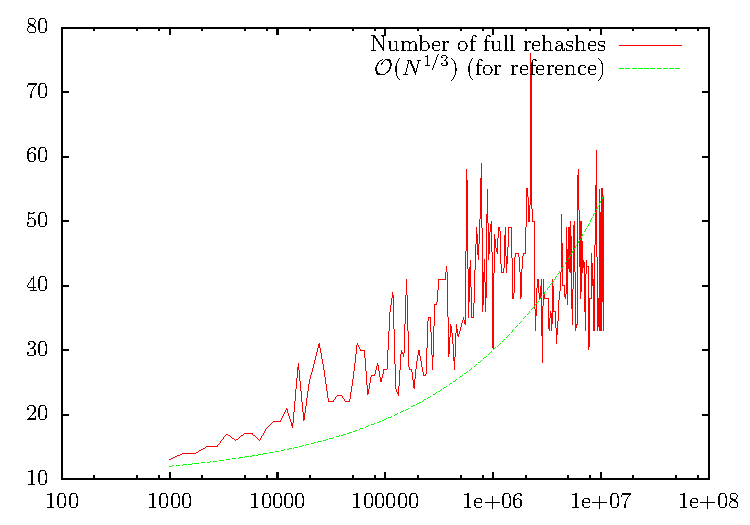
\includegraphics[width=0.7\textwidth]{img/cuckoo/results}
	\caption{Degenerate behavior of cuckoo hashing
		with simple tabulation ($\O(N^{1/3})$ rebuilds)
		as measured by our test program (\texttt{bin/experiments/cuckoo-cube}).}
\end{figure}

Examples of $\Theta(\log N)$-independent hashing schemes include:
\begin{itemize}
\item	For any $k$, a $k$-independent hash function family is \cite{new-hash-fns}:
	$$h(x)=\left(\sum_{i=0}^{k-1} a_i x^i \bmod p\right) \bmod M$$
	In this equation, $p$ is a prime greater than $|\mathcal{U}|$
	and all $a_i$ are chosen at random from $\Z_p$.
	This hash function family is considered slow due to needing
	$\Theta(\log N)$ time and using integer division by $p$.\footnote{%
		% TODO: This footnote looks like "p^2".
		As \cite{univ-classes} points out, using Mersenne primes
		(i.e.,\ $2^i-1$ for some $i$) enables a faster implementation of
		the modulo operation. On 64-bit keys, we could use $p=2^{89}-1$.
		It might not be possible to generalize this approach, because
		the question whether there are infinitely many Mersenne primes
		remains open.
	}
	Evaluation of this hash function takes $\O(k)$ steps on the RAM.
\item \cite{tab-based-4uni-hashing} presents a $k$-universal scheme that splits
	$x$ into $c$ components (as in simple tabulation hashing),
	expands $x$ into a \emph{derived key} $z$ of $\O(ck)$ components,
	and then applies simple tabulation hashing to $z$:
	$h(x)=\bigoplus h_i(z_i)$.
	When applied in our setting, where $c$ is fixed and $k=\O(\log N)$,
	the scheme takes time $\O(k)$ to evaluate.
	According to the authors, the scheme also has very competitive speed.
\item In order to outperform B-trees on the RAM, we would like to use a hashing
	function which evaluates faster than $\log N$. A scheme from
	\cite{univ-ext-random} needs only $\O(1)$ time to evaluate. Unfortunately,
	constructing a hash function by this scheme has high constant
	factors, so it is not very practical \cite{pagh-phd}.
\end{itemize}

% Both schemes need $\O(N^\epsilon)$ space to store the function.
% Drawback: large precomputed tables. CW-trick just requires $a_0,\ldots a_k-1$

For simplicity, our implementation of cuckoo hashing uses simple tabulation
hashing. As shown in section~\ref{sec:hashing-results}, \textsc{Insert}s were
significantly slower than with linear probing. Our work could be extended by
trying more sophisticated and more independent hash functions.

\section{Extensions of hashing}
Several methods have been developed for maintaining hash tables in an external
memory setting without expensive rehashing. some are presented in chapter 9
of~\cite{em-ads}.

In \cite{kirsch2009more}, cuckoo hash tables are extended with a small
constant-sized \emph{stash} (e.g., 3 or 4 items), which lowers the probability
of build failures and enhances performance (both theoretically and practically).

Cuckoo hashing can be generalized to more than two subtables.
The \textsc{Insert} procedure then performs slot eviction via a random walk.
According to \cite{open-questions-cuckoo}, experiments suggest that cuckoo
hash tables with more functions may be significantly more effective than simple
cuckoo hashing on high load factors. For example, 3 subtables perform well
with loads up to 91\%. However, more subtables would lead to more potential
cache misses in \textsc{Find} on large hash tables.

\chapter{B-trees}
\label{chapter:btree}
The B-tree is a very common data structure for storing sorted dictionaries.
They were introduced in 1970 as a method of efficiently maintaining ordered
indexes \cite{btree}.
B-trees are particularly useful where the external memory model is accurate,
because all information in every transferred block is actively used
in searching. For example, the ext4, Btrfs and NTFS filesystems use B-trees
to store directory contents and the MongoDB and MariaDB databases use B-trees
as indexes.  % TODO: Cite this claim.
Red-black trees, which are (in the left-leaning variant
described by \cite{left-leaning}) isomorphic to B-trees for $b=2$, are
commonly used to maintain in-memory dictionaries, for example in the GNU ISO
\Cpp Library as the implementation of the \texttt{std::map} STL template.
B-trees are also an optimal sorted dictionary data structure
for the external memory model assuming the only operation allowed on
keys is comparison.

B-trees are a generalization of balanced binary search trees.
Nodes of a B-tree keep up to $2b$ key-value pairs in sorted order.
An inner node of a binary search tree with key $X$ contains two pointers
pointing to children with keys $< X$ and $\geq X$. In B-trees,
inner nodes contain $k\in[b;2b]$ keys $K_1\ldots K_k$. There are $k+1$
child pointers in internal nodes: one for every interval
$[K_1;K_2),\ldots [K_{k-1};K_k)$, plus one for $(-\infty;K_1)$ and
$(K_k;\infty)$ each.
Leaf nodes of a B-tree store $[b;2b]$ key-value pairs.

B-trees can store values for keys either within all nodes (internal or leaves),
or only in leaves. If values are stored only in leaves, keys stored
within internal nodes are only used as pivots, and may not necessarily
have a value within leaves -- if a key is deleted, it is removed from its leaf
along with its node, but internal nodes may retain a copy of the key.
Our implementation stores values only inside leaves to allow tighter packing
of internal nodes.

The essence of the $[b;2b]$ interval is that when we try to insert
the $(2b+1)$-th key, we can instead split the node into two valid nodes of size
$b$ and borrow the middle key to insert the newly created node into the parent.
Similarly, when we delete the $b$-th key, we first try to borrow some nodes
from neighbours to create two valid nodes of size $[b;2b]$, which works when
there are at least $2b$ keys in both nodes combined.
When there are $2b-1$ keys, we instead bring down one key from the parent
and combine the two neighbours with the borrowed key into a new valid node with
$b+(b-1)+1=2b$ keys.

In binary search trees, searching for a key $K$ is performed by binary search.
Starting in the root node, we compare $K$ with the key stored in the node
and we go left or right depending on the result. If the current node's key
equals $K$, we fetch the value from the node and abort the search.

The process of finding a key-value pair in a B-tree generalizes this
by picking the child pointer corresponding to the only range that contains
the sought key $K$. To pick the child pointer, we can either do a simple
linear scan in $\Theta(b)$, or we can use binary search to get
$\Theta(\log b)$ if $b$ is not negligible.
Once we reach a leaf, we scan its keys and return the value for $K$
(if such a value exists).

To \textsc{Insert} a key-value pair in a B-tree, we first find the right
place to put the new key-value pair, and then walk back up the tree.
If an overfull node (with $> 2b$ keys) is encountered, it is split
to two nodes of $\leq b$ keys. One of the keys from the split node
is inserted to the parent along with a pointer to the new node.
When we split the root node, we immediately create a new root node above the
two resulting nodes.

Deletions employ a similar procedure: if the current node is underfull
(i.e.,\ if it has $< b$ keys), it is merged with one of its siblings.
If there are not enough keys among the siblings for two nodes,
one of the siblings takes ownership of all keys and the other sibling
is recursively deleted from the parent. In this case, the corresponding
key from the parent is pulled down into the merged node.
The only exception is the root node, which may have $[1;2b]$ keys.
If deleting from the root would leave the root with only one child
(and zero keys), we instead make the only child of the root the new root.

For B-trees that store values within both internal nodes and leaves,
some deletions will need to remove a key used as a pivot within an internal
node. In this case, the deleted key needs to be replaced by the minimum of its
left subtree, or the maximum of its right subtree.
Since our implementation stores values only inside leaves, deletions will
always start at a leaf, which slightly simplifies them.

Thus, updates to the B-tree keep the number of keys of all nodes within
$[b;2b]$, so the depth of the tree is kept between $\log_2b N$ and $\log_b N$
and the \textsc{Find} operation takes time
$\Theta(\log b \cdot \log_b N)=\Theta(\log N)$ and $\Theta(\log_b N)$
block transfers. \textsc{FindNext} and \textsc{FindPrevious} also take time
$\Theta(\log N)$, but if they are invoked after a previous \textsc{Find}, we
can keep a pointer to the leaf containing the key and accordingly adjust it to
find the next or previous key, which runs in $\O(1)$ amortized time. Thus,
B-trees also allow scanning a contiguous range of keys of size $k$ in
$\Theta(\log_b N + k)$ time.

The \textsc{Insert} and \textsc{Delete} operations may spend up to
$\Theta(b)$ time splitting or merging nodes on each level, so they run in
time $\Theta(b \cdot \log_b N)$.

The main benefit of B-trees over binary trees is the tunable parameter
$b$, which we can choose to be $\Theta(B)$. Practically, if the B-tree
is stored in a disk, $b$ can be tuned to fit one B-tree node in exactly one
physical block. Thus, in the external memory model, \textsc{Find},
\textsc{Insert} and \textsc{Delete} all take $\O(1)$ block transfers
on every level, yielding $\Theta(\log_B N)$ block transfers per operation.

This is optimal assuming the only allowed operation
on keys is comparison: reading a block of $\Theta(B)$ keys will only
give us $\log B$ bits of information, since the only useful operation
can be comparing the sought key $K$ with every key we retrieved.
We need $\log N$ bits to represent the index of the key-value pair we found,
so we need at least $\log N/\log B=\log_B N$ block transfers.

\chapter{Splay trees}
Splay trees are a well-known variant of binary search trees introduced
by \cite{splay} that adjust their structure with every operation, including
lookups. Splay tree operations cost $\O(\log n)$ amortized time, which is
similar to common balanced binary search trees, like AVL trees or
red-black trees.
However, unlike balanced search trees, splay trees adjust their structure
according to the access pattern, and the running time of a sufficiently long
sequence of \textsc{Find} operations on a splay tree is within a constant
factor of an optimal static search tree.
Thus, splay trees perform better than balanced search trees on non-uniform
access patterns, which are common in real-world applications.
Additionally, the \textit{dynamic optimality conjecture} proposes that
the performance of splay trees on a sequence of operations (including updates)
is within a constant factor of any dynamic search tree tailored for
the particular operation sequence.

TODO: disadvantage - slow individual operations, lots of local adjustments

TODO: copied.

Splay trees are binary search trees. A binary tree contains nodes, each of which
contains one key $K$ and its associated value.
A node has up to two children - a left one and a right one.
The left subtree contains only keys smaller than $K$ and the right subtree
contains only keys larger than $K$.

% To find a key $K$ in a binary search tree, we use binary search:
% we compare $K$ with the key in the tree's root and continue to the subtree
% that may contain $K$. If the current node has no child for us to descend into,
% the tree doesn't contain $K$.

Splay trees use a heuristic called \textit{splaying}, which moves a specified
node to the root of the tree by performing a sequence of rotations along the
path from the root to this note. Every rotation costs $\O(1)$ time and preserves
the left-to-right order of nodes in the binary search tree.

\begin{figure}
\centering
TODO: figure jako splay-trees.pdf (see page 4)
\caption{Left and right rotation of the edge between $x$ and $y$.}
%\label{fig:rotation}
\end{figure}

Splaying proceeds up from a node $x$ until $x$ is the root by performing
the following \textit{splaying step}.

Splaying step:
Denote the splayed node by $x$, its parent by $p$ and its grandparent by $g$.

Case 1 (zig): If $p$ is the root, rotate the $px$ edge. (This case is terminal)

Case 2 (zig-zig): If $p$ is not the root and $x$ and
		$p$ are both left or both right children, rotate
		the $gp$ edge, then rotate the $px$ edge.

Case 3 (zig-zag): If $p$ is not the root and $x$ is a left child and $p$
		is a right child (or vice versa), rotate the edge $px$ and
		then rotate the edge now joining $g$ with $x$.

\begin{figure}
\centering
TODO: figure jako splay-trees.pdf (see page 5)
\caption{The three cases of a splaying step up to left-right symmetry --
	zig, zig-zig and zig-zag.}
%\label{fig:splay-step}
\end{figure}

Splaying a node $x$ of depth $d$ takes $\Theta(d)$ time, which is the same
as the time to access $x$ from the root.
% Splaying reduces the depth of every node along the access path by roughly
% one half. TODO: fakt? TODO: figure

To \textsc{Find} a key in a splay tree, we try to find it using the general
search algorithm for binary search trees. If the search succeeds, we splay
up the node containing the key. Otherwise, we splay up the last visited
node.
An \textsc{Insert} is similar - we find the right place for the new node,
insert it, and finally splay it up.

% TODO: make it so 
\textsc{Delete}s are slightly more complex. We splay up the node to delete.
If it has one child, we delete it and replace it by its child. If it has
two children, we replace its value by the value of the right subtree's
leftmost node. Then we delete the right subtree's leftmost node, which has at
most 1 child by definition.

All update operations on splay trees take time $O(\log n)$.

To analyze the performance of the \textsc{Splay} operation, let us assign
a fixed positive weight $w(K)$ to every key $K$. Define the size $s(x)$
of a node $x$ to be the sum of all $w(K)$ for all keys $K$ in the node's
subtree and define the rank $r(x)$ of $x$ to be $\log s(x)$.
For amortization, let us define the potential $\Phi$ of the tree to be
the sum of the ranks of all its nodes.
We will measure the time to splay a node in the number of rotations done
(or 1 if we didn't perform any rotations).

% TODO: to je lemma
\begin{lemma}
The amortized time to splay a node $x$ in a tree with root
$t$ is $3(r(t)-r(x))+1 = \O(\log(s(t)/s(x)))$.
\end{lemma}
\begin{proof}
If there were no rotations, the bound is immediate. Thus suppose there is at
least one rotation. Consider any splaying step.
Let $s$ and $s'$, $r$ and $r'$ denote the size and rank functions just before
and just after the step, respectively. We show that the amortized time for
the step is at most $3(r'(x)-r(x))+1$ in case 1 and at most $3(r'(x)-r(x))$
in case 2 or case 3. Let $p$ be the original parent of $x$ and $g$ the original
grandparent of $x$ (if it exists).

Case 1 (zig):
	We perform only one rotation between $x$ and $p$.
	This rotation may only change the rank of $x$ and $p$, so
	the amortized time for this step is $1 + r'(x) + r'(p) - r(x) - r(p)$.
	Because $r(p)\geq r'(p)$, the amortized time is $\leq 1+r'(x)-r(x)$.
	Finally, since $r'(x)\geq r(x)$, the amortized time is also
	$\leq 1+3(r'(x)-r(x))$.

Case 2 (zig-zig):
	We perform two rotations that may change the rank of $x$, $p$
	and $g$, so the amortized time for the zig-zig step is
	$2+r'(x)+r'(y)+r'(z)-r(x)-r(y)-r(z)$. The zig-zig step
	moves $x$ to the original position of $g$, so $r'(x)=r(g)$.
	Before the step, $x$ was $p$'s child, and after the step,
	$p$ was $x$'s child, so $r(x)\leq r(p)$ and $r'(p)\leq r'(x)$.
	Thus the amortized time for this step is at most $2+r'(x)+r'(g)-2r(x)$.
	We claim that this is at most $3(r'(x)-r(x))$, that is, that
	$2r'(x)-r(x)-r(g)\geq 2$.

	$2r'(x)-r(x)-r'(g)=-\log\frac{s(x)}{s'(x)}-\log\frac{s'(g)}{s'(x)}$.
	We have $s(x)+s'(g)\leq s'(x)$.

	The $\log$ function is concave, so
	if $a,b\geq 0$ and $a+b\leq 1$, $\log a + \log b$ is maximized
	by setting $a = b = \frac{1}{2}$, which yields the value $-2$.
	Thus the inequality above is correct and the amortized time is
	at most $3(r'(x)-r(x))$.

Case 3 (zig-zag):
	The amortized time of the zig-zag step is
	$2+r'(x)+r'(p)+r'(g)-r(x)-r(p)-r(g)$. $r'(x)=r(g)$ and $r(x)\leq r(p)$,
	so the time is $\leq 2+r'(p)+r'(g)-2r(x)$.
	We claim that this is at most $2(r'(x)-r(x))$, i.e.
	$2r'(x)-r'(p)-r'(g)\geq 2$. This can be proven
	similarly to case 2 from the inequality $s'(p)+s'(g)\leq s'(x)$.
	Thus the amortized time for a zig-zag step is at most
	$2(r'(x)-r(x))\leq 3(r'(x)-r(x))$.

By telescoping the sum of amortized time for all performed steps until
$x$ becomes the root $t$, we get an upper bound of $3(r'(t)-r(x))+1$
for the entire splaying operation.
\end{proof}

By choosing different assignments of $w(i)$, we can obtain several basic
results. Note that over any sequence of $m$ splay operations
the total potential $\Phi$ may only drop by up to $\sum_{i=1}^N \log(W/w(i))$
where $W=\sum_{i=1}^n w(i)$, since the size of the node containing $i$
is between $w(i)$ and $W$.

\begin{theorem}[Balance Theorem]
A sequence of $m$ \textsc{Find}s on an $n$-item splay tree takes time
$\O((m+n)\log n+m)$.
\end{theorem}
\begin{proof}
Assign $w(i) = \frac{1}{n}$ to every item $i$. The amortized
access time for any item is at most $3\log(n)+1$. We have $W=1$, so by
the previous observation the potential drops by at most $n\log n$ over
the access sequence. Thus the time for the access sequence is at most
$(3\log n+1)m + n\log n = \O((m+n)\log n + m)$.
\end{proof}

TODO: relate Balance theorem and costs of inserts and deletes

For any item $i$, let $q(i)$ be the number of accesses of $i$ in an access
sequence.
\begin{theorem}[Static Optimality Theorem]
If every item is accessed at least once, the the total access time is
$\O(m + \sum_{i=1}^n q(i)\log\frac{m}{q(i)})$.
\end{theorem}
\begin{proof}
Assign a weight of $q(i)/m$ to every item $i$. For any item $i$, its
amortized time per access is $3(r(t)-r(x))+1=-3r(x)+1=-3\log(s(x))+1\leq
	-3\log(w(x))=O(\log(m/q(i)))$.
Since $W=1$, the net potential drop over the sequence is at most
$\sum_{i=1}{n}\log(m/q(i))$. The result follows.
\end{proof}

TODO: dynamic optimality conjecture

Let us denote the indices of accessed items as $a_1, \ldots a_m$
in the order they occur, where $a_i \in \{1,\ldots n\}$.

\begin{theorem}[Static Finger Theorem]
Fix any item $i_f$. Then the total access time is $\O(n\log n + m +
\sum_{j=1}^m \log(|a_j-f|+1))$.
\end{theorem}
% Static finger theorem proof missing here.

For any access $j\in\{1,\ldots m\}$, let $t(j)$ be the number of different
items accessed since the last access of item $i_{a_j}$ or since the
beginning of the access sequence.
\begin{theorem}[Working Set Theorem]
The total access time is $\O(n\log n + m + \sum_{j=1}^m\log(t(j)+1))$.
\end{theorem}
% Proof missing here.

The balance theorem states that on a sufficiently long sequence, lookups in
the splay tree are as efficient as in any balanced search tree. The static
optimality theorem implies that the splay tree is as efficient as any fixed
search tree, including the optimum tree for the given sequence, since
it is known that any sequence of accesses on a binary search tree
takes time at least $\Omega(m+\sum_{i=1}^n q(i)\log(m/q(i)))$.
% TODO: cite: ABRAMSON, N. Information Theory and Coding. McGraw-Hill, New York, 1983.
The static finger theorem can be interpreted to mean that accessing keys
whose value is close to a recently accessed value is fast.
Finally, the working set theorem implies that most recently
accessed items (the "working set") are cheap to access, which
makes splay trees behave well when the access pattern exhibits temporal
locality.

\section{Implementation}


\section{???}
A drawback of splay trees is that accessing the $\O(\log N)$ amortized
nodes on the access path may incur an expensive cache miss for every node --
splay trees make no effort to exploit the memory hierarchy.
In contrast, lookups in B-trees and cache-oblivious B-trees
only cause up to $\Theta(\log_B N)$ cache misses, which is a multiplicative
improvement of $\log B$.

On the other hand, splaying automatically adjusts the structure of the splay
tree to speed up access to recently or frequently accessed nodes. By the
working set theorem, accessing a small set of keys is always fast, no matter
how big the splay tree is. While B-trees and cache-oblivious B-trees are
also faster on smaller working sets, the complexity of any access remains
$\O(\log_B N)$, so accessing a small working set is slower on larger
dictionaries.

\chapter{$k$-splay trees}
\label{chapter:ksplay}
Splay trees are useful for exploiting the regularity of access patterns.
On the other hand, they do not make good use of memory blocks -- every node
is just binary, so walking to a~node in depth $d$ takes $\O(\log d)$ block
transfers. B-trees improve this by a~factor of $\log B$ by storing more keys
per node.

Self-adjusting $k$-ary search trees (or \emph{$k$-splay trees}) developed
by \cite{ksplay-sherk} use a~heuristic named \emph{$k$-splaying}
to dynamically adjust the structure of a~$k$-ary search tree according to
the query sequence. We have decided to implement and benchmark this data
structure because of the potential to combine self-adjustment for a~specific
search sequence with cache-friendly node sizes.

Similarly to B-trees, nodes in $k$-ary splay trees store up to $k-1$ key-value
pairs and $k$ child pointers. All nodes except the root are \emph{complete}
(i.e.\ they contain exactly $k-1$ pairs).

\mbox{B-tree} operations take $\Theta(\log_b N)$ node accesses. It can be
proven that \mbox{$k$-splay} tree operations need at most $\O(\log N)$
amortized node accesses, which matches ordinary splay trees, but unfortunately
$k$-splay trees do not match the optimal $\O(\log_k N)$ bound given by B-trees.
This conjecture from \cite{ksplay-sherk} was disproved in \cite{ksplay-nonopt},
where a~family of counterexample $k$-ary trees was constructed. For any $k$-ary
tree in this family, $k$-splaying a~key from a deepest node requires $\log N$
node accesses and produces another $k$-ary tree from the same family.

$k$-splay trees are proven in \cite{ksplay-sherk} to be $(\log k)$-competitive
compared to static optimal $k$-ary search trees.

The $k$-splaying operation is conceptually similar to splaying in the original
splay trees of Sleator and Tarjan, but $k$-splaying for $k=2$ differs from
splaying in original splay trees. To disambiguate these terms, we will
reserve the term \emph{splaying} for Sleator and Tarjan's splay trees and
we will only use \emph{$k$-splaying} to denote the operation
on $k$-ary splay trees.

In our description of $k$-splaying, we shall begin with the assumption that
all nodes on the search path are complete, and we will later modify
the $k$-splaying algorithm to allow \emph{incomplete} and \emph{overfull}
nodes.
Because splay trees store one key per node, it is not necessary to distinguish
between splaying a~node and splaying a~key. In $k$-ary splay trees, we always
$k$-splay nodes.

As with Sleator and Tarjan's splaying, $k$-splaying is done in steps.

Splaying steps of Sleator and Tarjan's splay trees involve 3 nodes connected
by 2 edges, except for the final step, which may involve the root node and one
of its children connected by an edge. In every step, the splayed node (or key)
moves from the bottom of a~subtree to the root of a~subtree.
Splaying stops when the splayed node becomes the root of the splay tree.

In $k$-splay trees, $k$-splaying steps involve $k$ edges connecting
$k+1$ nodes, except for the final step which may involve fewer edges.
The objective of $k$-splaying is to move a~\emph{star node} to the
root of the tree. In every $k$-splaying step, we start with the star node
at the bottom of a~subtree, and we change the structure of the subtree
so that the star node becomes its root.
The initial star node is the last node reached on a~search operation, and
$k$-splaying will move the content of this node closer to the root.
However, the structural changes performed in $k$-splaying steps shuffle
the keys and pointers of involved nodes, so after a~$k$-splay step,
the star node may no longer contain the key we originally looked up.
Unlike splay trees, the distinction between $k$-splaying a~node and a~key
is therefore significant.

There are two types of $k$-splay steps: \emph{non-terminal steps} on
$k+1$ nodes, and \emph{terminal steps} on less than $k+1$ nodes.
We consider first the non-terminal steps.

Non-terminal $k$-splay steps examine the bottom $k+1$ nodes in the search
path to the current star node. Denote the nodes $p_0,\ldots p_{k}$, where $p_i$
is the parent of $p_{i+1}$ and $p_k$ is the current star node. A~non-terminal
step traverses these nodes in DFS order and collects \emph{external children}
(i.e.\ children that are not present in $\{p_0,\ldots p_k\}$) and all key-value
pairs of $p_0,\ldots p_k$ in sorted order. These children and key-value pairs
are \emph{fused} into a~``virtual node'' with $(k+1)\cdot (k-1)$ keys and
$(k+1)\cdot(k-1) + 1$ children. Finally, this ``virtual node'' is broken down
into a~fully balanced $k$-ary search tree of depth 2. There is exactly one
way to arrange this $k$-ary search tree, because all its nodes must be complete.
The root of this search tree becomes the new star node and a~new $k$-splay
step starts.

Terminal $k$-splay steps occur when we are $k$-splaying at most $k$
nodes, with the highest one always being the root of the $k$-splay tree.
Unlike non-terminal steps, terminal steps have too few nodes in the splayed
path, so they leave the root underfull. Otherwise, terminal steps are the same
as non-terminal steps.

\begin{figure}
\centering
\begin{tikzpicture}[]
\tikzstyle{ks_node}=[rectangle split, rectangle split horizontal,
	rectangle split ignore empty parts, draw]
\tikzstyle{ks_leaf}=[circle, draw, text depth=0em, text height=0.5em, scale=0.9]

\node at (-4,0) [ks_node] {15 \nodepart{two} 95} [->]
child { node [ks_leaf] {a} }
child { node [ks_node] {21 \nodepart{two} 56}
	child { node [ks_leaf] {b} }
	child { node [ks_leaf] {c} }
	child { node [ks_node] {71 \nodepart{two} 80}
		child { node [ks_node] (StarBefore) {60 \nodepart{two} 64}
			child { node [ks_leaf] {d} }
			child { node [ks_leaf] {e} }
			child { node [ks_leaf] {f} }
		}
		child { node [ks_leaf] {g} }
		child { node [ks_leaf] {h} }
	}
}
child { node [ks_leaf] {i} };
\node at ($(StarBefore.west)+(-0.3,0)$) {$\star$};

\node at (4,-1.5) [ks_node] (StarAfter) {56 \nodepart{two} 71} [->]
child[sibling distance=2.5cm] { node [ks_node] {15 \nodepart{two} 21}
	child[sibling distance=0.7cm] { node [ks_leaf] {a} }
	child[sibling distance=0.7cm] { node [ks_leaf] {b} }
	child[sibling distance=0.7cm] { node [ks_leaf] {c} }
}
child[sibling distance=2.5cm] { node [ks_node] {60 \nodepart{two} 64}
	child[sibling distance=0.7cm] { node [ks_leaf] {d} }
	child[sibling distance=0.7cm] { node [ks_leaf] {e} }
	child[sibling distance=0.7cm] { node [ks_leaf] {f} }
}
child[sibling distance=2.5cm] { node [ks_node] {80 \nodepart{two} 95}
	child[sibling distance=0.7cm] { node [ks_leaf] {g} }
	child[sibling distance=0.7cm] { node [ks_leaf] {h} }
	child[sibling distance=0.7cm] { node [ks_leaf] {i} }
};
\node at ($(StarAfter.west)+(-0.3,0)$) {$\star$};

\draw[->] (-1,-1.5) -- (1,-1.5);

\end{tikzpicture}
\caption{Non-terminal 3-splaying step with marked star nodes.}
\end{figure}

\textsc{Delete} and \textsc{Insert} operations employ variations
of the same procedure. We look up the node to update and we insert or
delete the key within the node. Then, we $k$-splay the node, while allowing
the star node to be temporarily overfull or underfull. After $k$-splaying
the updated node, the root becomes the star node. If it has only one
child, we merge it with the root, and if the root has more than $k$ children,
we split it.

By performing an analysis similar to splay trees, \cite{ksplay-sherk}
shows that the number of node reads performed in a~sequence of $m$
\textsc{Find}s in a~$k$-splay tree with $N$ keys is
$\O(m\log N+\frac{N}{k}\log N)$.

\chapter{$k$-forests}
\label{chapter:kforest}
The performance of $k$-splay trees may suffer on access sequences chosen
by an adversary: it is known that certain access sequences must
take $\Omega(\log N)$ block transfers per element.
In 1991, \cite{martel} developed \emph{$k$-forests} --
a self-adjusting dictionary data structure based on a sequence of
$k$-ary search trees of increasing size.

The $k$-forest allows \textsc{Find}, \textsc{Insert} and \textsc{Delete}
operations in $\O(\log_k N)$ block transfers in the worst case. A simpler
randomized version of the data structure achieves the same expected bound.
It can be proven that a generalization of the Static Optimality theorem
also applies to $k$-forests: an element with access probability $p$
will have average lookup time $\O\left(\min\{\log_k \frac{1}{p}, \log_k
N\}\right)$. $k$-forests also have the working set property.

On the other hand, $k$-forests do not have fast finger queries. Scanning
a~\mbox{$k$-forest} in increasing key order takes $\Omega(N\log_k N)$.
Furthermore, all successor or predecessor queries take $\Omega(\log_k N)$
block transfers.

We are unaware of any data structure providing good speed for both static
searches and finger queries with a $\log_B$ reduction in block transfers
over splay trees.

A $k$-forest containing $N$ elements is a sequence of $\O(\log_k N)$ $k$-ary
search trees $T_1, T_2, \ldots$. Each tree $T_i$ contains up to $s(i)$ key-value
pairs, where $s(i) = k^{2^i} - 1$. The trees need to support $\O(\log_k s(i))$
time, so B-trees are a natural choice.

Every tree, with the possible exception of the last one, is kept full,
so tree $T_1$ has height 1, $T_2$ has height 2, $T_3$ has height 4, and so on.
Each key-value pair inserted into the data structure is always kept in one
tree $T_i$. The self-adjusting operation moves elements between trees to
keep more recently accessed elements in lower, smaller trees.
A deterministic version of this operation keeps the $s(1)$ most recently
accessed items in tree $T_1$, then the next $s(2)$ most recently accessed
items in $T_2$, and so on.

To \textsc{Find} a key, we scan the trees $T_i$ in increasing order of $i$.
If we scan all trees and find no matches, the search is unsuccessful.
Otherwise, the key-value pair is removed from its tree $T_i$ and inserted
into $T_0$. We then \emph{demote} one item from tree $T_0$ to $T_1$,
then from $T_1$ to $T_2$, and so on until all trees meet their size bounds.

\cite{martel} describes two implementations of \emph{demotion}.
The first one is a deterministic implementation named \emph{LRU demotion},
which maintains information about the time of last access to elements
in every tree. The element pushed down to the next tree is always the least
recently accessed one, so the trees $T_1,T_2,\ldots$ are maintained in sorted
order with respect to last access time.
A simpler implementation without auxiliary data is \emph{random demotion},
which simply selects a random key from $T_i$ to demote to $T_{i+1}$.
Both are equivalent in the sense that the expected time bounds arising
from random demotion equal the deterministic time bounds of LRU demotion.

\textsc{Insert} and \textsc{Delete} operations are similar to \textsc{Find}.
\textsc{Insert} inserts to $T_1$ and then demotes elements from $T_1,T_2,\ldots$
until the forest is fixed.
\textsc{Delete} finds the pair in its tree $T_i$ and removes it, and
then promotes items from all trees $T_{i+1},T_{i+2},\ldots$
Since both \textsc{Insert} and \textsc{Delete} need to promote and demote items
in potentially every tree $T_i$, they both access $\O(\log N)$ nodes.

As in our description of splay trees, let $K$ be the set of keys,
let $\{k_i: i\leq M\}$ be the sequence of indexes of accessed keys and
for any $j\in\{1,\ldots M\}$, let $t(j)$ be the number of distinct
keys accessed since the last access of key $K_{k_j}$.
\cite{martel} proves the following theorems analogous to desirable properties
of splay trees:
\begin{theorem}[Working Set Theorem for $k$-forests]
	With LRU demotion, the $j$th lookup accesses $\O(\log_k t(j))$ nodes.
	With random demotion, it accesses expected $\O(\log_k t(j))$ nodes.
\end{theorem}

Again, let $q(K_i)$ be the number of accesses of $K_i$.
\begin{theorem}[Static Optimality Theorem for $k$-forests]
	Accessing a sequence of keys $\{K_{k_i}: i\leq M\}$ requires
	$\O(\sum_{i=1}^N q(K_i) \log_k \frac{M}{q(K_i)})$ node accesses.
\end{theorem}

We implemented $k$-forests with random demotion to benchmark their performance,
especially to examine the constant multiplicative factors taken by promoting
and demoting in every operation.

\section{Related results}
\cite{alternatives-to-splay-trees} and \cite{unified-access-bound} extend
$k$-forests to build data structures with the \emph{unified property},
which is a strong generalization of the dynamic finger property and the working
set property of splay trees.
It is not known whether splay trees also have the unified property.
The data structure from \cite{alternatives-to-splay-trees} also improves
upon splay trees by guaranteeing a worst-case access time of $\O(\log N)$.
Unfortunately, the structure (as described by the authors) is static and highly
complex: each node of the structure stores 21 pointers.

\cite{dynamic-optimality-for-sl} uses a similar doubly exponential construction
to build a self-adjusting skip list. Operations on this skip list take time
$\O(\log t(j))$, which matches the working set bound on splay trees.
This structure is also shown to be dynamically optimal among skip lists
constrained by some restrictions (e.g.\ allowing at most $b$ consecutive forward
steps on any level for a fixed $b$), which implies that this restriction of
skip lists does not allow better performance than $\O(\log t(j))$.
Skip lists in this \emph{SL-B model} can be simulated in B-trees via
a construction from \cite{exploring-duality}. This representation yields
a B-tree that is dynamically optimal within a restricted class in the external
memory model. We are not aware of any implementations or benchmarks of this
data structure.
% TODO: more?

\chapter{Cache-oblivious B-trees}
\label{chapter:cob}
% TODO: assume B > 1
% TODO: usual => good? best?
% TODO: reference to B-tree article
The \emph{cache-oblivious B-tree} introduced by \cite{cobt}
is a data structure which replicates the asymptotic performance of B-trees
in a cache-oblivious setting.
\textsc{Find}s and updates on cache-oblivious B-trees require $\Theta(\log_B N)$
\footnote{Strictly speaking, the bound is $\Theta(1+\log_B N)$
	because we perform $\O(1)$ block transfers even when $B\in\omega(N)$.
	We decide to use the reasonable assumption that
	$B<N$ to simplify some bounds in this section.}
amortized block transfers, which is similar to cache-aware B-trees.
Scanning a range of $t$ keys also takes $\Theta(\log_B N+t/B)$ time.
% TODO: unfortunately not common for internal memory

The original cache-oblivious B-tree as described in \cite{cobt} used
weight-balanced B-trees. We implement a simplified version of the structure
from \cite{brodal01}, which is composed of three components.
% TODO: nevadi ze tady jsou data obracene?
The \emph{van Emde Boas layout} of binary trees is a way of cache-obliviously
maintaining full binary trees in memory such that reading or updating any
root-to-leaf path in root-to-leaf or leaf-to-root order takes $\Theta(\log_B N)$
block transfers.
Then, the \emph{packed memory array} lets us store a ``cache-oblivious linked
list''. The items of this ``linked list'' will represent key-value pairs.
% TODO: previous sentence not really true
The packed memory array has fast updates in the amortized sense. Inserting
and deleting items overwrites $\Theta(\frac{\log^2 N}{B})$ amortized memory
blocks.
Finally, we combine the two previous parts with \emph{indirection} to obtain
the desired $\Theta(\log_B N)$ time to \textsc{Find}, \textsc{Insert} and
\textsc{Delete}.

\section{The van Emde Boas layout}
The van Emde Boas layout is a way of mapping the nodes of a full binary
tree of height $h$ to indices $0\ldots 2^h-2$. Other layouts of full binary
trees include the BFS or DFS order.

Surprisingly, the van Emde Boas layout was not invented by van Emde Boas.
The name comes from the earlier \emph{van Emde Boas priority queue},
which was invented by \citeauthor{van-emde-boas} in \citeyear{van-emde-boas}.
The van Emde Boas priority queue uses a height splitting scheme similar
to the van Emde Boas layout. The cache-oblivious application of this idea
was devised in \cite{veb-layout}.

The advantage of storing a full binary tree in the van Emde Boas layout
is that is lets us read the sequence of keys from the root to any leaf
using $\Theta(\log_B N)$ block transfers, which matches the \textsc{Find}
cost of B-trees without the need to know $B$ beforehand.
In contrast, the same operation would cost $\Theta(\log N-\log B)$ block
transfers in the DFS or BFS order.

The van Emde Boas layout is defined recursively. To find the van Emde Boas layout
of a full binary tree of height $h$, we split the tree to bottom subtrees
of height $\lhfloor h-1 \rhfloor$ and one top subtree of height $h - \lhfloor
h-1 \rhfloor$.
The subtrees are recursively aligned in the van Emde Boas layout and then laid
out: the top tree first, followed by the bottom trees in BFS order.
The van Emde Boas layout of a one-node tree is trivial.

\begin{figure}
\centering
\begin{tikzpicture}[
	every node/.style={inner sep=0, outer sep=0},
	level 1/.style = {sibling distance=7.1cm},
	level 2/.style = {sibling distance=3.5cm},
	level 3/.style = {sibling distance=1.7cm},
	level 4/.style = {sibling distance=0.8cm},
	veb_node/.style = {align=center, inner sep=0pt, text centered, circle,
		font=\sffamily, draw=black, text width=1.2em, outer sep=0pt},
	block_l0/.style = {rectangle, draw=black, dashed, inner sep=0.2cm,
		draw=gray},
	block_l1/.style = {rectangle, draw=black, densely dotted, thin, inner
		sep=0.1cm, draw=gray},
	level/.style={level distance=1.2cm}
]
	\node [veb_node] (Node0) {0}
	child{ node [veb_node] (Node1) {1}
		child { node [veb_node] (Node2) {2}
			child { node [veb_node] (Node4) {4}
				child { node [veb_node] (Node5) {5} }
				child { node [veb_node] (Node6) {6} }
			}
			child { node [veb_node] (Node7) {7}
				child { node [veb_node] (Node8) {8} }
				child { node [veb_node] (Node9) {9} }
			}
		}
		child { node [veb_node] (Node3) {3}
			child { node [veb_node] (Node10) {10}
				child { node [veb_node] (Node11) {11} }
				child { node [veb_node] (Node12) {12} }
			}
			child { node [veb_node] (Node13) {13}
				child { node [veb_node] (Node14) {14} }
				child { node [veb_node] (Node15) {15} }
			}
		}
	}
	child{ node [veb_node] (Node16) {16}
		child { node [veb_node] (Node17) {17}
			child { node [veb_node] (Node19) {19}
				child { node [veb_node] (Node20) {20} }
				child { node [veb_node] (Node21) {21} }
			}
			child { node [veb_node] (Node22) {22}
				child { node [veb_node] (Node23) {23} }
				child { node [veb_node] (Node24) {24} }
			}
		}
		child { node [veb_node] (Node18) {18}
			child { node [veb_node] (Node25) {25}
				child { node [veb_node] (Node26) {26} }
				child { node [veb_node] (Node27) {27} }
			}
			child { node [veb_node] (Node28) {28}
				child { node [veb_node] (Node29) {29} }
				child { node [veb_node] (Node30) {30} }
			}
		}
	};

	\node [block_l0,fit=(Node0)] (BlockT) {};
	\node [block_l0,fit=(Node1) (Node5) (Node15)] (BlockB0) {};
	\node [block_l0,fit=(Node16) (Node20) (Node30)] (BlockB1) {};

	\node [block_l1,fit=(Node1) (Node2) (Node3)] (BlockB0T) {};
	\node [block_l1,fit=(Node4) (Node5) (Node6)] (BlockB0B0) {};
	\node [block_l1,fit=(Node7) (Node8) (Node9)] (BlockB0B1) {};
	\node [block_l1,fit=(Node10) (Node11) (Node12)] (BlockB0B2) {};
	\node [block_l1,fit=(Node13) (Node14) (Node15)] (BlockB0B3) {};

	\node [block_l1,fit=(Node16) (Node17) (Node18)] (BlockB1T) {};
	\node [block_l1,fit=(Node19) (Node20) (Node21)] (BlockB1B0) {};
	\node [block_l1,fit=(Node22) (Node23) (Node24)] (BlockB1B1) {};
	\node [block_l1,fit=(Node25) (Node26) (Node27)] (BlockB1B2) {};
	\node [block_l1,fit=(Node28) (Node29) (Node30)] (BlockB1B3) {};
\end{tikzpicture}
% TODO: linearized figure, general figure

\caption{The van Emde Boas layout of a full binary tree of height 5.
Boxes mark recursive applications of the construction. Note that the indices
within every box are contiguous, so at some level of detail, reading
a box will take $\O(1)$ block transfers.}
\label{fig:veb_layout_5}
\end{figure}

\begin{theorem}
In a tree stored in the van Emde Boas layout, reading the sequence of nodes
on any root-leaf path costs $\Theta(\log_B N)$ block transfers.
\end{theorem}

\begin{proof}
Let us examine the recursive applications of the van Emde Boas construction
for a height $h=\log (N+1)$. Denote the heights of the bottom trees
$h_1, h_2, \ldots$. For example, as seen in Figure \ref{fig:veb_layout_5}, for
$h=5$ we have $h_1=4$, $h_2=2$ and $h_3=1$.

Let us assume that the entire tree doesn't fit in a block of size $B$.
Because we can assume that a single node fits in one block, there exists a \emph{level of
detail} $i$ such that the $2^{h_i}-1$ nodes in $i$-th-iteration bottom trees
fit in a block of size $B$, while bottom trees of $i-1$-th-iteration bottom
trees do not.

Since $2^{h_i}-1 < B$ and $2^{h_i-1}-1 \geq B$, it follows that $h_i=\O(\log_B N)$.
By construction, the path of from the root of the tree to any leaf contains
$\Theta(\log N/h_i)=\Theta(\log_B N)$ bottom trees from the $i$-th iteration.
The path also contains one top tree, which includes the root.
As seen on Figure \ref{fig:veb_layout_5}, this top tree may have a height
different than $h_i$, but the height of this tree is always $\leq h_i$.

Because the $2^{h_i}-1$ nodes of any $i$-th-iteration bottom tree are stored
in contiguous memory, every $i$-th-iteration bottom tree (or top tree)
can be read using $\O(1)$ block transfers. Since every root-to-leaf path
is composed of $\Theta(\log_B N)$ such subtrees, traversing the path
takes $\Theta(\log_B N)$ block transfers (plus $\O(1)$ in the uncommon
case when $B > N$).
\end{proof}

The van Emde Boas layout thus makes a fine data structure for querying static
data, but it does not allow inserting or deleting nodes. We will need
to combine it with another data structure to allow updates.

\subsection{Efficient implementation of implicit pointers}
A useful property of the van Emde Boas layout is that it is fully specified
by $h$ of the tree, so there is no need to keep pointers to child nodes.
The positions of left and right children of a node can be calculated from
$h$ when they are needed.
This is particularly useful when $B$ is small and when the size of pointers
is similar to the size of keys, because not storing pointers lets us
effectively use a higher branching factor than B-trees with explicit
pointers could.
For example, if we store 8-byte keys in a B-tree and if we align nodes to
a 64-byte cache line, each node can only store up to 3 keys. In contrast,
64 bytes of a van Emde Boas layout store 8 keys.
% We refer to this property of the layout as allowing
% \emph{implicit pointers}.

We will only use the van Emde Boas order to walk in the direction from
the root node to a leaf or in reverse.
Given the \emph{van Emde Boas ID} of a node (denoted as numbers
inside the nodes in Figure \ref{fig:veb_layout_5}),
we can easily calculate the van Emde Boas IDs of its children by
a recursive procedure. This procedure either returns \emph{internal} node
pointers, referencing actual nodes of the tree, or it returns \emph{external}
indexes, which represent virtual nodes below the leaves, counted from left
to right.

\begin{algorithmic}
\Function {GetChildren} {$n$: node van Emde Boas ID, $h$: tree height}
	\If {$h = 1$ and $n = 0$} \Return{external (0,1)} \EndIf

	\State {$h_\downarrow \gets \lhfloor h-1 \rhfloor$} \Comment{Calculate
top and bottom heights}
	\State {$h_\uparrow \gets h-h_\downarrow$}
	\State {$N_\uparrow, N_\downarrow \gets 2^{h_\uparrow}-1,
	2^{h_\downarrow}-1$} \Comment{Calculate top and bottom tree sizes}

	\If {$n <  N_\uparrow$}
		\State $\ell, r \gets$ \Call{GetChildren}{$n$,$h_\uparrow$}
		\If {$\ell$ and $r$ are internal}
			\State \Return{internal ($\ell$,$r$)}
		\Else\Comment{$\ell$ and $r$ point to bottom tree roots}
			\State \Return{internal
				($N_\uparrow+\ell\cdot N_\downarrow$,
				$N_\uparrow+r\cdot N_\downarrow$)
			}
		\EndIf
	\Else
		\State {$i \gets (n-N_\uparrow) \div N_\downarrow$}
			\Comment{The node $n$ lies within the $i$-th bottom tree.}
		\State {$b \gets N_\uparrow + i\cdot N_\downarrow$}
			\Comment{$b$ is the root of the $i$-th bottom tree.}
		\State $\ell,r\gets$ \Call{GetChildren}{$n-b$, $h_\downarrow$}
		\If {$\ell$ and $r$ are internal}
			\State \Return{internal ($\ell+b$, $r+b$)}
		\Else
			\State {$e \gets 2^{h_\downarrow}$} \Comment{Adjust
				indices by $e$ external nodes per bottom
				tree.}
			\State \Return{external ($\ell+i\cdot e$, $r+i\cdot e$)}
		\EndIf
	\EndIf
\EndFunction
\end{algorithmic}

The cost of this procedure in the cache-oblivious model is $\O(1)$, because
it can be implemented using constant memory by modifying the tail recursion into
a loop. Unfortunately, on a real computer, this is not quite the case --
every call of this procedure performs $\Theta(\log\log N)$ instructions and
the cost of calling this procedure $\Theta(\log N)$ times between the root
and a leaf is not negligible compared to the cost of memory transfers.
Indeed, this calculation of implicit pointers can become the performance
bottleneck of the cache-oblivious B-tree.
This can be slightly alleviated by caching the results for trees of small
height, which allows us to stop the recursion early.

As described in \cite{brodal01}, at the low cost of precomputing $\O(h)$
items for every height $h$ of the binary tree, we can perform root-leaf
traversals in constant time per traversed level.

The main observation is that for any node in a fixed depth $d$,
performing the recursive construction until the selected node is the root
of a bottom tree will progress through the same sizes of top and bottom trees.

For every depth $d\in[2;h]$, let us precompute the size $B[d]$ of
bottom trees rooted in depth $d$, the size $T[d]$ of the corresponding
top tree and the depth $D[d]$ of the top tree's root. The data takes $\O(\log
N)$ memory and it can be computed in $\O(\log N)$ time by an iterative procedure.
Table \ref{tab:depth_data_example} shows the values of these arrays
for the 5-level van Emde Boas layout shown in figure \ref{fig:veb_layout_5}.

\begin{table}[h]
	\centering
	\begin{tabular}{r|r|r|r}
		$d$ & $B[d]$ & $T[d]$ & $D[d]$ \\
		\hline
		0   & --     & --     & --     \\
		1   & 15     & 1      & 0      \\
		2   & 1      & 1      & 1      \\
		3   & 3      & 3      & 1      \\
		4   & 1      & 1      & 3
	\end{tabular}
	\caption{$B[d]$, $T[d]$ and $D[d]$ for the 5-level van Emde
	Boas layout.}
	\label{tab:depth_data_example}
\end{table}

While traversing a root-to-leaf path, we shall maintain the depth
$d$ of the current node $X$, the index $i$ of the current node in BFS order
and an array $Pos[j]$ of van Emde Boas order indices of nodes passed in every
depth $j<d$ during this traversal.

As the bits of the BFS index $i$ correspond to left and right turns made during
the traversal, the $\log(T[d]+1)$ least significant bits of $i$ are the
index of the unique bottom tree rooted by the node $X$. Because $T[d]$ is
always in the form $2^k-1$, we can find those bits quickly by calculating
$i \And T[d]$.

Because the current node $X$ is the root of the $(i \And T[d])$-th
bottom tree of size $B[d]$ after a top tree of size $T[d]$ rooted in
$Pos[D[d]]$, it follows that the van Emde Boas index of the current node can be
calculated in $\O(1)$ time as:
$$Pos[d]=Pos[D[d]] + T[d] + (i \And T[d]) \cdot B[d]$$

Our root-to-leaf traversal starts by setting $i\gets 0, d\gets 0, Pos[0]=0$.
Navigation to the left or right child of the current node is performed
by updating the BFS index $i$ (setting it to $2i+1$ or $2i+2$ respectively),
incrementing the depth $d$ and calculating the new $Pos[d]$.
We can also return one level higher by reversing the update of $i$ and
decrementing $d$.

In our root-to-leaf traversals, reading the value of a non-leaf node $N$ will be
followed by reading the value of its right child $R$. Based on the value in
$R$, we will then either descend further below $R$, or we will descent into
the subtree below $N$'s left child $L$.
We can slightly optimize this access pattern by calculating $Pos[d]$ for $L$
from $Pos[d]$ for $R$ by simply subtracting $T[d]$, because $B[d]$ will
decrease by 1. This saves us one relatively expensive multiplication
instruction whenever moving to the left sibling.

\begin{figure}
\centering
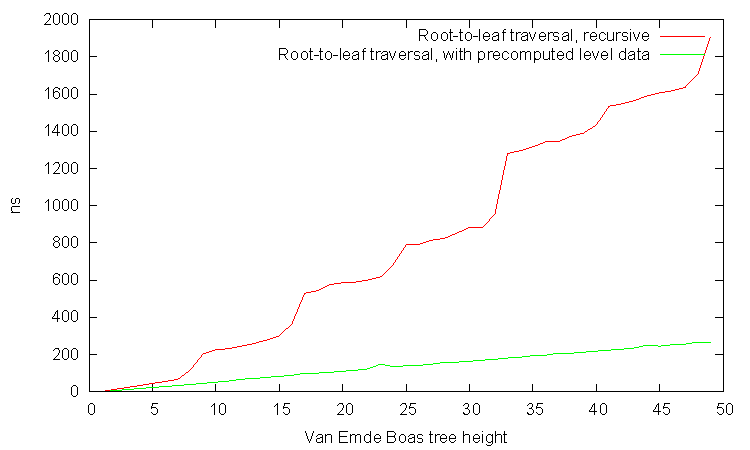
\includegraphics{img/veb-drilldown-speed}
\caption{Average time for computing node pointers in root-to-leaf traversals
	of van Emde Boas layouts, implemented trivially and with precomputed
	level data.}
\label{fig:veb_drilldown_speed}
\end{figure}
As evident in figure \ref{fig:veb_drilldown_speed}, using precomputed level data
saves a considerable amount of computation, especially with deeper van Emde Boas
layouts.

\section{Ordered file maintenance}
Ordered file maintenance algorithms maintain $N$ items stored in a physical
array of size $\O(N)$. Aside from reading from any slot in the array,
we can ask the algorithm to \textsc{Insert} a new item before or after
a given index in the array, and \textsc{Delete}(\emph{index}), which deletes
the item at a given index. Updates are allowed to move elements of the array,
but the relative order of all stored items must remain the same.

While the interface is similar to a simple linked list, storing the items
in a contiguous array of size $\O(N)$ lets us scan a range of size $k$ using
only the optimal $\Theta(k/B)$ scans, which improves upon linked lists by
a factor of $B$.

To give the maintenance algorithm some freedom, empty gaps of up to a constant
maximum size may be present between two adjacent items in the array. Without
gaps, \textsc{Insert} and \textsc{Delete} would have to be implemented
by shifting elements to the right or left in $\Theta(N/B)$ block transfers.

The \emph{packed memory array} is a data structure that maintains an ordered
file. Updates (\textsc{Insert}s and \textsc{Delete}s) of a packed memory array
rewrite a contiguous range of amortized size $\Theta(\log^2 N)$.
Thanks to the range being contiguous, updates will incur
$\Theta(\frac{\log^2 N}{B})$ amortized block transfers.

The array is divided into logical \emph{leaf blocks} of constant size
$\O(\log N)$. A \emph{virtual full binary tree} is built above those leaf
blocks. Every node of this binary tree represents the range covering all
the leaf blocks below. This tree is only conceptual -- it is never stored
in memory.

To properly define the structure, we need to define some terms. The
\emph{capacity} of a certain range of the array is its size and the
\emph{density} of a range is the number of items present in the range divided
by its capacity.
The packed memory array maintains certain bounds on the densities of subranges
of the array.

The densities in the leaf blocks are kept between \unichar{"00BC} % VULGAR FRACTION ONE QUARTER
and 1. If an update keeps the density of the leaf block within thresholds,
we perform the update by rewriting all $\Theta(\log N)$ items of the leaf block.
When a block becomes too sparse or too dense, we walk up the binary
tree until we find a node that fits our density requirements.
Walking up the binary tree corresponds to ``multiplying the range by two''
to the left or to the right.

The density requirements become stricter as we walk up the virtual tree.
In particular, the density of a node of depth $d$ within a tree of height $h$
is kept between $\frac{1}{2}-\frac{1}{4}\frac{d}{h}$ and $\frac{3}{4}+\frac{1}{4}\frac{d}{h}$
\footnote{The constants are arbitrary and control the tradeoff
between memory consumption and time complexity of rebuilding.}.
When we find a node that is \emph{within threshold}, we uniformly redistribute
the items in its range. If no such node exists, we resize the entire structure
by a constant factor, which lets us amortize the costs of this resizing to
a multiplicative constant.

We claim that while this redistribution may reorganize a range of size up
to $\O(N)$, the redistribution of a node puts all nodes below it well within
their thresholds, so the next reorganization will be needed only after many more
updates.
% TODO: how much is "many"?

The search for a node to redistribute is implemented as two interspersed scans,
one extending the scanned range to the left, one to the right. The
redistribution can be done by collecting all items in the array on the left side
of the array using a left-to-right scan, followed by a right-to-left scan
putting items into their final destinations. Thus,
redistributing a range of $K$ items takes $\Theta(K/B)$ block transfers.

TODO: figure of redistribution

\begin{theorem}
The block-transfer cost of an update of the packed-memory array
is $\Theta(\frac{\log^2 N}{B})$ amortized.
\end{theorem}

\begin{proof}
Suppose we need to redistribute some node $X$ of depth $d$ after performing
an insertion. Since we are redistributing this node, it is within threshold,
but one of its children, say $Y$, is not.
Therefore the density of $X$ is at most
$\frac{3}{4}+\frac{1}{4}\frac{d}{h}$, while the density of $Y$ is more than
$\frac{3}{4}+\frac{1}{4}\frac{d+1}{h}$. After we redistribute the items within $X$,
the density of $Y$ will drop by $\frac{1}{h}$. Thus, if we denote the capacity
of $Y$ as $|Y|$, we will need to insert at least $|Y|/h$ items under any
child of $X$ before we need to rebalance $X$ again.
Thus, we can charge the $\O(|X|)$ cost of redistributing $X$ to the
insertions into $Y$, which gives us amortized $\O(\log N)$
redistribution steps per insertion into $Y$.

Since the node $Y$ has $h=\Theta(\log N)$ ancestors, we can amortize
$\Theta(\log N \cdot \log N)$ redistribution steps per insertion, which is
$\Theta(\frac{\log^2 N}{B})$ in block transfers. The proof of the deletion
cost is analogous.
\end{proof}

\section{Cache-oblivious B-tree}
The first step of constructing a cache-oblivious B-tree is a bootstrapping
structure, which is a combination of a full binary tree in
the van Emde Boas layout and the packed memory array.
The packed memory array stores inserted key-value pairs sorted by the key.
Nodes of the tree map to ranges in the array, with leaves mapping
to individual slots and the root mapping to the entire ordered file.
The nodes of the tree contain dictionary keys.
Leaves store the keys stored in their corresponding ordered file slots,
or $\infty$ if the slot is empty. Each internal node of the tree
stores the minimum of its subtree.

\begin{figure}
\centering
\newcommand{\guide}[1]{
	\path[thin, draw=gray] (veb_#1) -- ($(#1,1)+(-0.5,0)$);
}
\begin{tikzpicture}[
	pma_empty/.style = {very thin, draw=gray, cross out, scale=1.5},
	veb/.style = {scale=0.8, minimum size=0.8cm, draw, circle, align=center},
	pma_full/.style = {}
	level 0/.style = {sibling distance=8cm},
	level 1/.style = {sibling distance=4cm},
	level 2/.style = {sibling distance=2cm},
	level 3/.style = {sibling distance=1cm},
]
\draw[step=1cm] (0,0) grid (8,1);
\node[pma_full] at (+0.5,+0.5) (pma_1) {1};
\node[pma_empty] at (+1.5,+0.5) (pma_2) {};
\node[pma_empty] at (+2.5,+0.5) (pma_3) {};
\node[pma_full] at (+3.5,+0.5) (pma_4) {6};
\node[pma_full] at (+4.5,+0.5) (pma_5) {25};
\node[pma_empty] at (+5.5,+0.5) (pma_6) {};
\node[pma_full] at (+6.5,+0.5) (pma_7) {53};
\node[pma_full] at (+7.5,+0.5) (pma_8) {102};

\node[veb] at (4,5) {1}
[level distance=1cm]
child{ node [veb] {1}
	child { node [veb] {1}
		child { node [veb] (veb_1) {1} }
		child { node [veb] (veb_2) {$\infty$} }
	}
	child { node [veb] {6}
		child { node [veb] (veb_3) {$\infty$} }
		child { node [veb] (veb_4) {6} }
	}
}
child{node [veb] {25}
	child { node [veb] {25}
		child { node [veb] (veb_5) {25} }
		child { node [veb] (veb_6) {$\infty$} }
	}
	child { node [veb] {53}
		child { node [veb] (veb_7) {53} }
		child { node [veb] (veb_8) {102} }
	}
};

\guide{1}; \guide{2}; \guide{3}; \guide{4};
\guide{5}; \guide{6}; \guide{7}; \guide{8};

\end{tikzpicture}
\caption{The bootstrapping structure of the cache-oblivious B-tree}
\end{figure}

\textsc{Find}ing a key in the bootstrapping structure is done by binary search
on the tree. The binary search either finds the ordered file slot which contains
the key-value pair, or it finds an empty slot. Either way, walking down
the tree costs $\Theta(\log_B N)$ block transfers.

\textsc{Insert}s and \textsc{Delete}s first walk to the position the key
would normally occupy, using $\Theta(\log_B N)$ block transfers. The key
is then inserted into the ordered file, which costs
$\Theta(\frac{\log^2 N}{B})$ block transfers. Finally, the tree needs to be
updated to reflect the reorganization of the packed memory array.

TODO: update analysis: VEB update

This bootstrapping structure matches B-trees in the speed of \textsc{Find},
but updates take time $\Theta(\log_B N+\frac{\log^2 N}{B})$, which is
$\Theta(\frac{\log^2 N}{B})$ more than B-trees.
This matches the performance of B-trees for $B=\Omega(\log N\log\log N)$.
Unfortunately, this is not a realistic assumption in internal memory
where cache lines are relatively small, so we need to remove the
$\Theta(\frac{\log^2 N}{B})$ term to fully match B-trees.

To remove this term, we will use this bootstrapping data structure with
\emph{indirection} to make the final cache-oblivious B-tree.

The final \emph{cache-oblivious B-tree} will store key-value pairs
partitioned into \emph{pieces} in disjoint intervals. A piece is an array of
$P=\Theta(\log N)$ slots, which contains between $P/4$ and $P$ key-value pairs.
% TODO: opravdu? ne spis 3/4P? to bych mel overit...
Since pieces are physical arrays, reading or fully rewriting a piece
takes $\Theta(\frac{\log N}{B})$ block transfers.
The \emph{bootstrapping structure} stores pointers to the $\Theta(N/\log N)$
pieces as values, keyed by their minimal keys.

\begin{figure}
\centering
\newcommand{\guide}[1]{
	\path[thin, draw=gray] (veb_#1) -- ($(#1,1)+(-0.5,0)$);
}
\begin{tikzpicture}[
	pma_empty/.style = {very thin, draw=gray, cross out, scale=1.5},
	veb/.style = {scale=0.8, minimum size=0.8cm, draw, circle, align=center},
	pma_ptr/.style = {fill, scale=0.3, circle}
	level 0/.style = {sibling distance=8cm},
	level 1/.style = {sibling distance=4cm},
	level 2/.style = {sibling distance=2cm},
	level 3/.style = {sibling distance=1cm},
]
\draw[step=1cm] (0,0) grid (8,1);
\node[pma_ptr] at (+0.5,+0.5) (pma_1) {};
\node[pma_empty] at (+1.5,+0.5) (pma_2) {};
\node[pma_empty] at (+2.5,+0.5) (pma_3) {};
\node[pma_ptr] at (+3.5,+0.5) (pma_4) {};
\node[pma_ptr] at (+4.5,+0.5) (pma_5) {};
\node[pma_empty] at (+5.5,+0.5) (pma_6) {};
\node[pma_ptr] at (+6.5,+0.5) (pma_7) {};
\node[pma_ptr] at (+7.5,+0.5) (pma_8) {};

\node[veb] at (4,5) {1}
[level distance=1cm]
child{ node [veb] {1}
	child { node [veb] {1}
		child { node [veb] (veb_1) {1} }
		child { node [veb] (veb_2) {$\infty$} }
	}
	child { node [veb] {6}
		child { node [veb] (veb_3) {$\infty$} }
		child { node [veb] (veb_4) {6} }
	}
}
child{node [veb] {25}
	child { node [veb] {25}
		child { node [veb] (veb_5) {25} }
		child { node [veb] (veb_6) {$\infty$} }
	}
	child { node [veb] {53}
		child { node [veb] (veb_7) {53} }
		child { node [veb] (veb_8) {102} }
	}
};

\node[inner sep=0] at (0.5,-2) (bucket1) {
	\begin{tikzpicture}
	\draw[step=0.8cm] (0,0) grid (0.8,-2.401);
	\node at (+0.4,-0.4) {1};
	\node at (+0.4,-1.2) {3};
	\node at (+0.4,-2.0) {5};
	\end{tikzpicture}
};

\node[inner sep=0] at (3.5,-1.2) (bucket2) {
	\begin{tikzpicture}
	\draw[step=0.8cm] (0,0) grid (0.8,-0.801);
	\node at (+0.4,-0.4) {6};
	\end{tikzpicture}
};

\node[inner sep=0] at (4.5,-1.6) (bucket3) {
	\begin{tikzpicture}
	\draw[step=0.8cm] (0,0) grid (0.8,-1.601);
	\node at (+0.4,-0.4) {25};
	\node at (+0.4,-1.2) {41};
	\end{tikzpicture}
};

\node[inner sep=0] at (6.5,-2.0) (bucket4) {
	\begin{tikzpicture}
	\draw[step=0.8cm] (0,0) grid (0.8,-2.401);
	\node at (+0.4,-0.4) {53};
	\node at (+0.4,-1.2) {58};
	\node at (+0.4,-2.0) {92};
	\end{tikzpicture}
};

\node[inner sep=0] at (7.5,-1.2) (bucket5) {
	\begin{tikzpicture}
	\draw[step=0.8cm] (0,0) grid (0.8,-0.801);
	\node at (+0.4,-0.4) {102};
	\end{tikzpicture}
};

\path[->,>=latex] (pma_1) edge (bucket1.north);
\path[->,>=latex] (pma_4) edge (bucket2.north);
\path[->,>=latex] (pma_5) edge (bucket3.north);
\path[->,>=latex] (pma_7) edge (bucket4.north);
\path[->,>=latex] (pma_8) edge (bucket5.north);

\guide{1}; \guide{2}; \guide{3}; \guide{4};
\guide{5}; \guide{6}; \guide{7}; \guide{8};

\end{tikzpicture}
\caption{Full cache-oblivious B-tree with indirection}
\end{figure}

To \textsc{Find} a key in the cache-oblivious B-tree, we walk down the
bootstrapping structure in $\Theta(\log_B (N/\log N))=\Theta(\log_B N)$
to find the piece that may contain the key, and scan it in
$\Theta(\frac{\log N}{B})$, so we still need only $\Theta(\log_B N)$
block transfers for \textsc{Find}s.
\textsc{FindNext} and \textsc{FindPrevious} work similarly.

\textsc{Insert}s and \textsc{Delete}s first find the appropriate piece
to update in $\Theta(\log_B (N/\log N))$. If the piece can be updated
without getting under $P/4$ or over $P$ items, we rewrite the piece in
$\Theta(\frac{\log N}{B})$, removing or inserting the key. If we changed
the minimum of the piece, we also need to walk up the tree in $\Theta(\log_B
(N/\log N))$ to propagate the change.

If the piece is too full, we split the piece into two pieces of size
$P/2$. The splitting takes $\Theta(\frac{\log N}{B})$ block transfers.
Afterwards, the new piece needs to be inserted to the bootstrapping structure
in $\Theta(\frac{\log^2 (N/\log N)}{B})$ amortized transfers.
Similarly, if the piece is too sparse, we merge the piece with one of its
neighbors. A neighbor can be found in $\O(1)$, because the pieces are
stored in the packed memory array, which guarantees gaps of constant size.
If the two pieces have more than $3P/4$ items, we only ``borrow'' some keys from
the neighbor and update the bootstrapping structure in $\Theta(\log_B N)$
to reflect new piece minima.
If there are less than $3P/4$ items in total, the pieces get merged and one
of them will be deleted from the bootstrapping structure in
$\Theta(\frac{\log^2 (N/\log N)}{B})$.

Thus, updates take $\Theta(\log_B N)$ plus $\Theta(\frac{\log^2 N}{B})$
every time we need a split or a merge. However, we don't need splits and
merges too often: splitting a full piece creates two pieces of size $P/2$,
which will be only split or merged again after $\Theta(P)$ more updates.
Merging two pieces yields a piece with between $P/2$ and $3P/4$ items.
This new piece will also be updated only after $\Theta(P)$ more updates.
Thus, we can charge each update $\Theta(\frac{1}{\log N}\frac{\log^2 N}{B})$
for splits and merges, which gives us $\Theta(\log_B N+\frac{\log N}{B})=
\Theta(\log_B N)$ amortized time for updates.

Finally, updates may necessitate a change in piece size $P$. If $P$
no longer fits, we pick a new $P$ by adding or subtracting a small constant
$\Delta_P$ and we globally rebuild the structure.
Because piece sizes need to change after the data structure increases
or decreases in size by a factor of $2^{\Delta_P}$, we can allow
rebuilds to take up to $\Theta(N\log_B N)$ block transfers -- the amortized
cost of rebuilds will be $\O(1)$ per item.
% TODO: rebuilding smart might maybe take just $\Theta(N/B)$ block transfers?

\section{Enhancements}
An alternative deamortized ordered file maintenance data structure
developed by \cite{willard92} performs $\Theta(\frac{\log^2 N}{B})$
block transfers in the worst case. A cache-oblivious B-tree backed by this
structure would limit the worst-case number of block transfers from
$\Theta(\frac{N}{\log N})$ to just $\Theta(\frac{\log^2 N}{B}+\log_B
N)$ while keeping the amortized bound at $\Theta(\log_B N)$.

% TODO: Should I mention this?
% \footnote{
% 	In a practical implementation, the worst-case bound needs an additional
% 	$\frac{N}{B}$ term to account for necessary reallocations of
% 	the backing array once it becomes too full.}

As we observed with applying the van Emde Boas layout, removing auxiliary
data can greatly speed up operations -- the tree in van Emde Boas layout has
half the effective depth of a B-tree, because cache lines can fit more keys
when pointers are implicit.
\emph{Implicit data structures} are designed to waste as little memory on
auxiliary information as possible. Implicit dictionaries are allowed to only
store a permutation of the stored data and $\O(1)$ memory cells of additional
information. Bookkeeping information, such as pointers or small integers
of $b$ bits, is usually encoded by a pairwise permutation of $2b$ keys,
with $x_{2i} < x_{2i+1}$ corresponding to 1 and $x_{2i} > x_{2i+1}$
corresponding to 0.

\cite{implicit-btrees-survey} gives an overview of progress on implicit
dictionaries.  In \citeyear{implicit-cob}, \citeauthor{implicit-cob} reached
the optimal bound of $\Theta(\log_B N)$ block transfers per search or operation
in an implicit setting. Similarly to the simple cache-oblivious B-tree, their
construction uses the deamortized version of the packed memory array
in conjunction with the van Emde Boas layout. To avoid holes in the packed
memory array, the elements of the packed memory array are chunks of keys.
Several other modifications are necessary to allow updates in size, which
requires building the structure on the fly.
We decided not to implement the implicit cache-oblivious B-tree due
to its large complexity. We also believe the data structure may be much
slower on practical data sets than equivalent structures with free slots or
pointers, since decoding auxiliary data from the implicit representation
requires reading large permutations of keys.

\section{Notes on optimization}
TODO: this primarily serves as a place to put my notes.
I may eventually put some of this into the final text.

\subsection{Inlining of van Emde Boas drilldown hot spots}
See commit \texttt{76d4a6c}. The main Van Emde Boas drilldown
methods (\texttt{drilldown\_go\_left} and \texttt{drilldown\_go\_right})
were previously compiled in a separate module. Making them inline
in the header file increased cache-oblivious B-tree performance
by approximately 10\%.

\subsection{Removing double walking in COBT insertions}
See commit \texttt{2fcdee5dd}.
\texttt{cob\_insert} needs to test that the inserted key doesn't exist
in the data structure yet. The first version performed this by calling
\texttt{cob\_find} and then finding the leaf to insert into, inserting
and fixing the van Emde Boas tree. While the code was very easy to understand,
it also duplicated the step of finding the correct leaf, since it used
to be done first by \texttt{cob\_find} and then by \texttt{cob\_insert}.

Changing the code to first look up the leaf and then to test for key presence
and possibly insert the new key-value pair increased performance.

Tested on \texttt{bin/experiments/performance -m 10M -a dict\_cobt}:
Before: 111.93 107.52 108.41 108.59 114.54, after:
99.95, 101.05, 102.63, 102.41, 100.96.
The speedup is about 8\%.

\subsection{Keeping stack for splaying in \texttt{splay\_tree.c}}
See commit \texttt{90f9247}.
\texttt{splay\_tree\_insert} previously first added a new node, and then called
a separate function to find the new node by its key and to splay it up.
Constructing a "splay stack" while inserting enhanced performance by about 12\%.
Original \texttt{bin/experiments/performance -m 10M -b 5 -a dict\_splay}:
13.770, 13.589, 13.868. After: 12.348, 12.172, 12.15.

\chapter{Implementation}
To measure the performance of various data structures, we implemented them
in the C programming language (using the C11 revision).
We have chosen this language for several reasons:
\begin{itemize}
\item The language is low-level, which enables a high degree of tuning by hand.
	Our data structures are also not slowed down by common features of
	high-level languages, such as garbage collection.
\item C toolchains are mature and they can be expected to optimize code well.
\item The C language is very portable and most other languages can
	call C functions. This enables our data structures to be potentially
	easily used in other projects.
\end{itemize}

Our code was developed using the GNU C Compiler (version 4.9.2) on Linux.
We used the Git version control system, with our repository hosted at
\url{https://github.com/MichalPokorny/thesis}. The code includes a test suite,
which tests implementation details of particular data structures as well
as general fuzz tests for checking that implemented data structures behave
like proper dictionaries. We used Travis CI (\url{https://travis-ci.org/})
to automatically test our code after submission.

All dictionaries assume 64-bit keys and values (represented as the
\texttt{uint64\_t} type). It would be easy to allow keys and values of arbitrary
size, but such a choice would be likely to slow down operations on
the data structures, because a range of compiler optimizations would
be impossible in code assuming general lengths. For example, copying
keys and values would need to be a general loop or
\texttt{memcpy}/\texttt{memmove} call, while assuming a constant key/value
size of 64 bits lets us copy in one CPU instruction. Using the C++ language,
we could potentially use templates to make our data structures both general
and optimized. If we are willing to sacrifice some code style, we could
make the C code behave similarly by moving the implementation into a header
file, which could be configured to generate a general data structure
tuned to specific parameters prior to inclusion, as in the following example:
\begin{lstlisting}
struct my_value {
	uint64_t stuff[32];
};
#define IMPLEMENTATION_PREFIX myimpl
#define IMPLEMENTATION_KEY_TYPE uint64_t
#define IMPLEMENTATION_VALUE_TYPE struct my_value
#include "btree/general.impl.h"

void usage() {
	dict* btree;
	dict_init(&btree, &dict_myimpl_btree);
	// ...
}
\end{lstlisting}
For example, the LibUCW library (\url{http://www.ucw.cz/libucw/})
uses this pattern for generic binomial heaps and hash tables.
We have decided to forgo generality to keep the code clean and readable.

\section{General dictionary API}
All implemented data structures can be used through a common API defined
in \texttt{dict/dict.h}. To encapsulate implementation details from
users of the API, we have used a common C ``trick'', where we represent
dictionaries as ``virtual table pointers'' and ``private data''.
The common API represents a dictionary as a pointer to an opaque structure.
The type pointed to is declared in \texttt{dict/dict.h} as:
\begin{lstlisting}[language=C]
typedef struct dict_s dict;
\end{lstlisting}

The \texttt{struct dict\_s} structure is defined in \texttt{dict/dict.c}
to prevent exposure of implementation details from users including
\texttt{dict/dict.h}:
\begin{lstlisting}[language=C]
struct dict_s {
	void* opaque;
	const dict_api* api;
};
\end{lstlisting}

The \texttt{opaque} pointer is maintained by the concrete implementation.
\texttt{dict\_api} is a "virtual method table" type defined in
\texttt{dict/dict.h}:

\begin{lstlisting}[language=C]
typedef struct {
	int8_t (*init)(void**);
	void (*destroy)(void**);

	bool (*find)(void*, uint64_t key, uint64_t *value);
	int8_t (*insert)(void*, uint64_t key, uint64_t value);
	int8_t (*delete)(void*, uint64_t key);

	const char* name;

	// More function pointers.
} dict_api;
\end{lstlisting}

The \texttt{init} and \texttt{destroy} functions are passed a pointer to the
\texttt{opaque} pointer and they respectively initialize and deinitialize it.
The \texttt{name} field is a human-readable name of the data structure.
Other fields are given the \texttt{opaque} pointer as the first argument
and they act as implementations of their respective general versions operating
on general dictionaries declared in \texttt{dict/dict.h}:

\begin{lstlisting}[language=C]
bool dict_find(dict*, uint64_t key, uint64_t *value);
int8_t dict_insert(dict*, uint64_t key, uint64_t value);
int8_t dict_delete(dict*, uint64_t key);
\end{lstlisting}

Dictionary data structures may optionally implement successor and predecessor
lookups. The public API consists of the functions \texttt{dict\_next} and
\texttt{dict\_prev}. If the data structure does not implement these operations,
it may set the appropriate fields in \texttt{dict\_api} to \texttt{NULL}.
The \texttt{dict\_api\_allows\_order\_queries} and
\texttt{dict\_allows\_order\_queries} functions detect whether ordered
dictionary operations are available for the given implementation or dictionary.
\begin{lstlisting}[language=C]
bool dict_api_allows_order_queries(const dict_api*);
bool dict_allows_order_queries(const dict*);
bool dict_next(dict*, uint64_t key, uint64_t *next_key);
bool dict_prev(dict*, uint64_t key, uint64_t *prev_key);
\end{lstlisting}

Every data structure implementation exposes a global variable of type
\texttt{const dict\_api} named \texttt{dict\_mydatastructure}. For example,
a B-tree can be used as follows:

\begin{lstlisting}[language=C]
#include <inttypes.h>
#include <stdio.h>

#include "dict/btree.h"
#include "dict/dict.h"

void example_btree(void) {
	dict* btree;
	if (dict_init(&btree, &dict_btree) != 0) {
		printf("Error initializing B-tree.\n");
		return;
	}
	if (dict_insert(btree, 1, 100) != 0) {
		printf("Error inserting 1 -> 100.\n");
	}
	// ...
	const bool found = dict_find(btree, 42, &value);
	if (found) {
		printf("Found 42 -> \%" PRIu64 ".\n",
				value);
	} else {
		printf("No value for 42.\n");
	}
	// ...
	if (dict_delete(btree, 1) != 0) {
		printf("Failed to remove key 1.\n");
	}
	dict_destroy(&btree);
}
\end{lstlisting}

Finally, we have decided to reserve one key for internal purposes.
This key is defined in \texttt{dict/dict.h} as the macro
\texttt{DICT\_RESERVED\_KEY} and its value is \texttt{UINT64\_MAX}.
Inserting this key into a dictionary or deleting it will result in an error.
Reserving this value is useful for representing unused slots in B-tree
and $k$-splay tree nodes.

We implemented the following dictionary data structures:
\begin{itemize}
\item \texttt{dict\_array}, declared in \texttt{dict/array.h}:
	a sorted array of key-value pairs with $\O(N)$ insertions and deletions,
	indended as a benchmark on very small inputs.
\item \texttt{dict\_btree}, declared in \texttt{dict/btree.h}:
	a B-tree with nodes aligned to 64 B cache lines
	(Chapter~\ref{chapter:btree}).
\item \texttt{dict\_cobt}, declared in \texttt{dict/cobt.h}:
	a cache-oblivious B-tree (Chapter~\ref{chapter:cob}).
\item \texttt{dict\_htcuckoo}, declared in \texttt{dict/htcuckoo.h}:
	cuckoo hash table with simple tabulation hashing
	(Section~\ref{sec:cuckoo}).
\item \texttt{dict\_htlp}, declared in \texttt{dict/htlp.h}:
	an open-addressing hash table with linear probing and simple tabulation
	hashing (Section~\ref{sec:open-addressing}).
\item \texttt{dict\_splay}, declared in \texttt{dict/splay.h}:
	a splay tree (Chapter~\ref{chapter:splay}).
\item \texttt{dict\_ksplay}, declared in \texttt{dict/ksplay.h}:
	a $k$-splay tree (Chapter~\ref{chapter:ksplay}). % TODO: which K?
% TODO: htable
\end{itemize}

\section{Performance measurement}

% TODO: measure memory
Our goal is to have fast data structures with reasonable memory usage.
We measure the performance of the various dictionary implementations
on several experimental setups.

We tracked the time it took to conduct each experiment using the POSIX function
\texttt{clock\_gettime}. To better understand the bottlenecks, we also
tracked certain hardware events of interest using the \texttt{perf\_events} API
of the Linux kernel. This API is a generic wrapper around platform-specific
performance counters. Events such as cache misses or branch mispredictions
increment these counters.

TODO: track RAM
TODO: cite perf

\section{Synthetic experiments}
Each synthetic experiment setup has a tunable \emph{size} $S$
(i.e.\ the maximum number of stored key-value pairs needed by the experiment).
The synthetic setups include:
\begin{itemize}
\item
	\emph{Random inserts and finds}: We generate pseudorandom key-value
	pairs by applying two deterministic invertible functions $k(i)$
	and $v(i)$ for $i$ between 0 and $S-1$.
	These simple functions use a Feistel network to provide
	``sufficiently randomly behaving'' key-value pairs while letting us
	derive $i$ from $k(i)$ or $v(i)$, which aids debugging.

	After the pairs are inserted, they are read in an order determined
	by a simple pseudorandom generator with a fixed seed.

	On this experiment, we separately measure the performance of deletions
	and finds.

\item
	\emph{Left-to-right scans}: We seed the structure with $S$ items
	as above. Then we traverse the dictionary from the minimum key to
	the maximum key, reading the values as we go. We don't include
	the seeding in our measurements.
	Left-to-right scans are only available on implementations that
	allow predecessor and successor queries.

\item
	\emph{Working set patterns}: The working set experiment needs
	a fixed integer parameter $W<S$. We again randomly seed the dictionary
	with $S$ items. Finally, $S$ times we access the key-value pair
	with key $k(i)$, where $i$ is picked pseudorandomly from
	$\{0,\ldots,W-1\}$.
	This access pattern is intended to simulate datasets, which have
	a mostly-static ununiform access probability distribution.

\item
	\emph{Word occurrence counting}: We load a large text document
	and we tokenize it into words. Each word is then normalized
	to lowercase and transformed into a 64-bit integer via a simple
	hash function $h$. We create a dictionary storing counts of word
	occurrences keyed by word hashes. Each word $w$ is inserted into
	the dictionary by either inserting a new $\langle h(w), 1\rangle$ pair,
	or deleting an existing pair for $h(w)$ and inserting a new one
	with an incremented value.
	This usage pattern approximates building a search index on the document.
	TODO: which document?
\end{itemize}
The code of synthetic experiments is located in \texttt{experiments/performance}.

\section{Non-synthetic experiments}
\cite{libavl} surveys the performance of different binary search tree
implementations on concrete real-life workloads. In particular, splay trees
were reported to be several times faster than AVL or red-black trees when
maintaining virtual memory areas of the Mozilla browser, VMware or the Squid
HTTP proxy. The author also simulated the workload of the mapping from peer
IP addresses to IP datagram identification nonces. On this workload, splay
trees underperformed balanced search trees.

To investigate the practical performance of our data structure implementations,
we decided to collect recordings of dictionary access patterns in real programs
and to collect performance metrics on replays of these recordings.

\subsection{Mozilla Firefox}
The Mozilla Firefox web browser contains an unordered dictionary template class
named \texttt{nsTHashtable} in \texttt{xpcom/glue/nsTHashtable.h}.
The default implementation uses double hashing. The template class implements
the \textsc{Find}, \textsc{Insert} and \textsc{Delete} operations. Additionally,
it supports enumerating all key-value pairs in the structure in an arbitrary
order.

We placed simple logging into the implementations of \textsc{Find},
\textsc{Insert} and \textsc{Delete}. For simplicity, we did not log
enumerations. Except splay trees, every data structure we implemented
can be extended to implement arbitrary-order enumerations in $\O(N/B)$ block
transfers, so we believe the effect of enumerations on the relative performance
differences between data structures would be relatively small.

After a browsing session, we counted the number of operations logged
on every \texttt{nsTHashtable} instance and we selected the top 10
instances with most operations.

TODO: what about variable-length keys (folding)
TODO: what about values

Presumably for the sake of optimization, \texttt{nsTHashtable} has a more
liberal interface than we implemented. Aside from searches and updates,
\texttt{nsTHashtable} also supports enumerating all key-value pairs in
an arbitrary order (i.e.\ depending on the internal hash function).
The user is also allowed to update values in enumerated key-value pairs
at no extra \textsc{Find} cost.
We skipped arbitrary enumeration when replaying recorded operations.
Because further calls to \texttt{nsTHashtable} may depend on the arbitrary
order of enumeration, we expect that \texttt{nsTHashtable} would behave
better on recorded operations than any of our structures. For example,
since \texttt{nsTHashtable} will enumerate keys in the order in which they
are stored within \texttt{nsTHashtable}, \texttt{nsTHashtable} will reap
the rewards of cache friendliness, while our data structures will be much
more likely to read from unpredictable locations.

Fairly comparing data structures in the presence of arbitrary-order enumeration
would require actually running our source code within the instrumented program.
We did not pursue this direction further in this thesis, but benchmarking data
structures directly where they are used may provide inspiration for better
optimizations. Particularly interpreters of dynamic programming languages
with built-in dictionary types, like Python or Ruby, could prove interesting
test subjects.

\subsection{Geospatial database}
To test the performance of \textsc{FindNext} and \textsc{FindPrevious}, we
simulated the workload of a simple database of geospatial data supporting
local searching. The source code for this experiment is stored in
\texttt{experiments/cloud}. It can be built by running \texttt{make
bin/experiments/cloud}. Before running the experiment, input data must
be downloaded by running \texttt{./download.sh} from within
\texttt{experiments/cloud}.

We used data from \emph{Extended Edited Synoptic Cloud Reports from Ships and
Land Stations Over the Globe, 1952-2009 (NDP-026C)} (\cite{cloud-reports}).
The main part of this dataset consists of 196 compressed plaintext files
containing one cloud report per line. Aside from many other fields,
each report contains the date and UTC hour, the longitude and latitude of the
reporting ship or land station and the measured sea level pressure and
wind speed.
Our simulated database loads all air temperature and wind speed measurements
and indexes them by their coordinates. Given a position on the globe, the
database can return a set of reports taken close to the position.

To implement this database in the context of our general dictionary API,
we map from latitude-longitude pairs to dictionary keys via a
locality-preserving mapping called the \emph{Z-order} (or
\emph{Morton order} after its inventor, who introduced it in
\cite{morton-order}). The Z-order computes a one-dimensional key from
a position in multiple dimensions simply by interleaving the bits of
the coordinates. One-dimensional distances implied by the Z-order only
approximate the original two-dimensional distances, so the Z-order is
not useful for exact closest-point queries -- we only use it as an
approximation. For the sake of simplicity, we also interpret
latitude-longitude angles as plane coordinates, without any attempt
to merge 180\textdegree~W and 180\textdegree~E.

Because stations at one position usually give multiple reports,
the key for our dictionary also needs to contain a unique identifier of
the report, which we create by counting the reports from each unique position
and append after the Z-order code of the position.
Some stations also do not provide the wind speed or air pressure.
Records from stations which provide neither are not loaded, and records
with missing values are also skipped at query time.

\begin{figure}
\centering
\begin{tikzpicture}
\node at (0,0) (z_2x2) {\begin{tikzpicture}
	\draw[step=1cm,gray,very thin] (0,0) grid (2,2);
	% NOTE: TikZ coordinate system has (0,0) in bottom left.
	\draw[thick] (0.5,1.5) -- (1.5,1.5) -- (0.5,0.5) -- (1.5,0.5);
	\end{tikzpicture}
};
\node at (4,0) (z_4x4) {\begin{tikzpicture}
	\draw[step=1cm,gray,very thin] (0,0) grid (4,4);
	% NOTE: TikZ coordinate system has (0,0) in bottom left.
	\draw[thick] (0.5,3.5) -- (1.5,3.5) -- (0.5,2.5) -- (1.5,2.5) --
		(2.5,3.5) -- (3.5,3.5) -- (2.5,2.5) -- (3.5,2.5) --
		(0.5,1.5) -- (1.5,1.5) -- (0.5,0.5) -- (1.5,0.5) --
		(2.5,1.5) -- (3.5,1.5) -- (2.5,0.5) -- (3.5,0.5);
	\end{tikzpicture}
};
\end{tikzpicture}
\caption{Z-order in two dimensions}
\end{figure}

A possible alternative would be using a \emph{Peano curve}
(introduced in \cite{peano-curve}, later generalized into
\emph{Hilbert curves} of arbitrary dimension by \cite{hilbert-curve}).
A desirable property of Peano curves is that points mapped to adjacent
one-dimensional points are also adjacent in the multidimensional space.
We decided to use the Z-order for the simplicity of its mapping function.

Queries are implemented simply by mixed calls to \texttt{dict\_prev} and
\texttt{dict\_next} until we collect enough results. A non-toy database might
perform some additional filtering to ensure only reports within a certain
distance are returned.

Our usage of this simulated database will pick $S$ random points on the globe.
For each point, we fetch $R$ close records and we calculate the average
recorded sea-level atmospheric pressure and wind speed in these records.
Atmospheric pressures and wind speeds are packed into 64-bit values, which
are stored in the ordered dictionary.

\begin{figure}
\centering
\begin{subfigure}[b]{1.0\textwidth}
	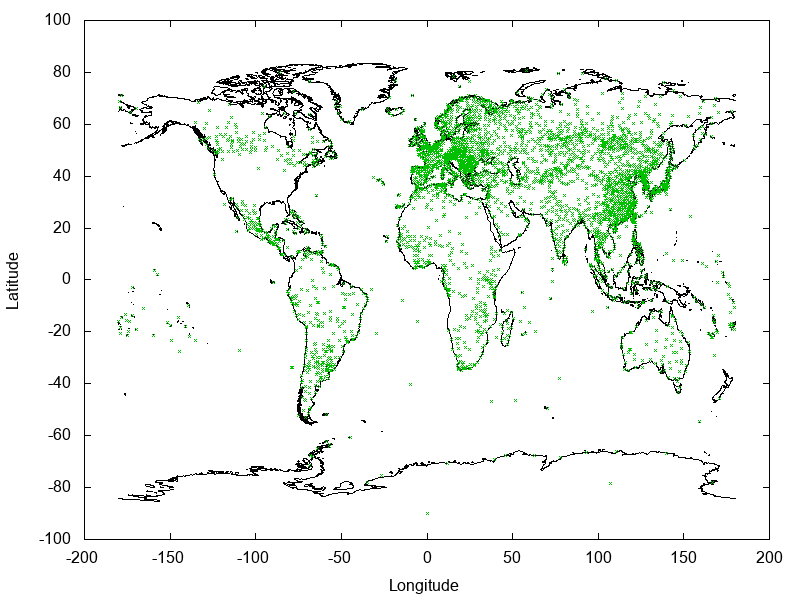
\includegraphics[width=\textwidth]{img/cloud/stations}
	\caption{Stations providing wind speed or air pressure data}
\end{subfigure}

\begin{subfigure}[b]{1.0\textwidth}
	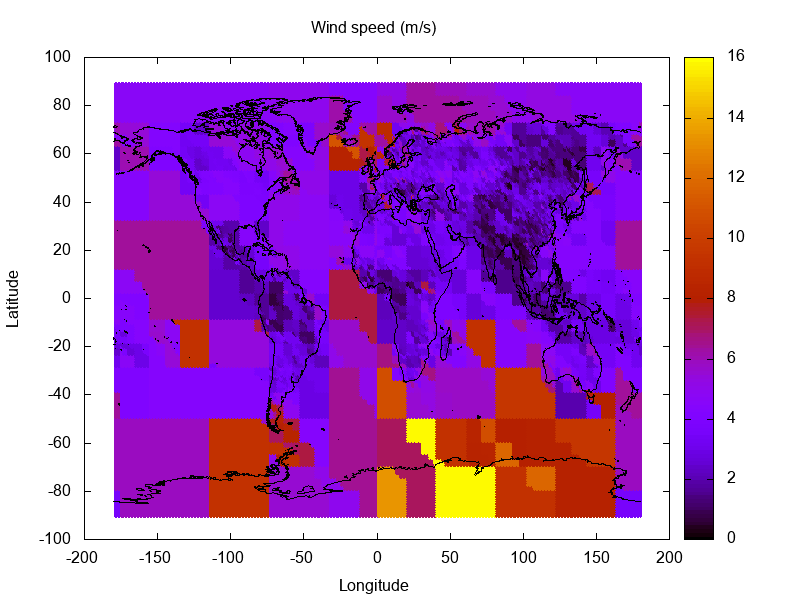
\includegraphics[width=\textwidth]{img/cloud/wind-speed}
	\caption{Average wind speeds}
\end{subfigure}
\end{figure}
\clearpage
\begin{figure}[H]
\centering
\ContinuedFloat
\begin{subfigure}[b]{1.0\textwidth}
	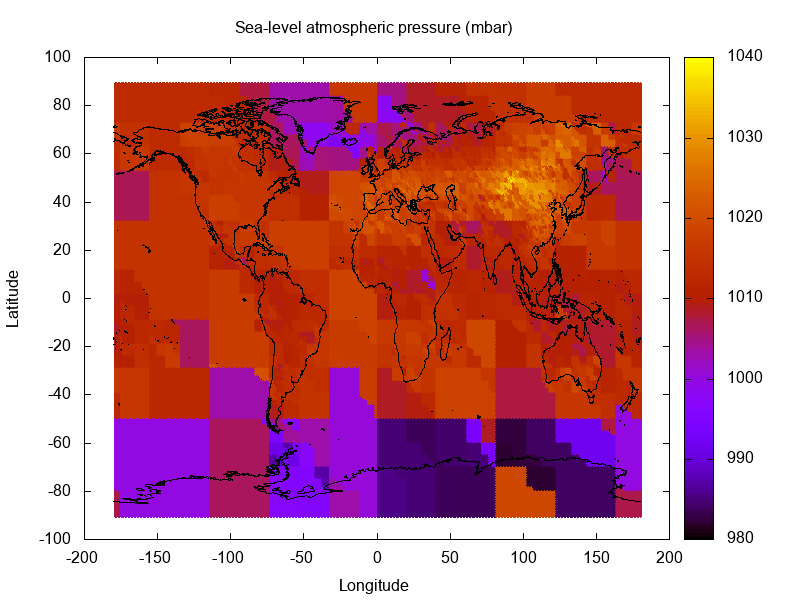
\includegraphics[width=\textwidth]{img/cloud/pressure}
	\caption{Average sea-level atmospheric pressure}
\end{subfigure}
\caption{Results from the cloud data experiment.
	Each query sampled 1000 close measurements.}
\end{figure}


\chapter*{Conclusion}
\addcontentsline{toc}{chapter}{Conclusion}

We confirmed that cache-oblivious B-trees are practically competitive with
more common data structures in main memory, especially on larger dictionaries
with frequent \textsc{Find}s and uniform access patterns.

Our implementation of $k$-splay trees and $k$-forests performed badly.
In our opinion, they alone are not a practical replacement for simple splay
trees. A more optimized implementation of $k$-splaying might reach parity with
splay trees.

Experiments on data recorded from Mozilla Firefox suggest that splay trees
and cuckoo hash tables do well on most dictionaries as they are practically
used. A particularly interesting conclusion that can be drawn from
Table~\ref{tab:firefox-results} is that hashing with linear probing may
be (somewhat counterintuitively) slower than splay trees.
Larger databases that require order queries also seem to be best served
by splay trees, followed by cache-oblivious \mbox{B-trees} and cache-aware
\mbox{B-trees}.

\section*{Suggestions for further research}
The dictionary problem is well-explored, including structures for efficient
in particular models of computation and practical libraries for real computers.
The space-time limitations of this thesis unfortunately did not permit us to
completely survey all of them.

We believe an benchmarking various non-traditional self-adjusting structures,
like tango trees from \cite{tango} or multi-splay trees from
\cite{multisplay-trees}, could give interesting results. Splay trees are very
performant on practical access patterns, but their worst-case $\O(N)$ behavior
limits their usefulness in time-sensitive systems. Some self-adjusting
structures provide better worst-case access times (e.g.\ $\O(\log N)$ in
multi-splay trees. On the other hand, the implementation of splay trees
are considerably simpler, so the complexity of operations might outweight
time saved by fewer cache misses in the worst case.

Several data structures based on tries have also been proposed for the
dictionary problem. One example are \emph{y-fast tries} \cite{y-fast},
which allow \textsc{Find}s in time $\O(1)$ and updates and predecessor/successor
queries in time $\O(\log\log |U|)$, where $U$ is the key universe. They require
$\O(N \log\log |U|)$ memory.
The RAM model is required by y-fast tries -- they assume that RAM operations
can be performed on keys in constant time.
The original motivation for developing y-fast tries was lowering the memory
requirements of van Emde Boas queues ($\O(|U|)$) while keeping the same time
for operations.
% TODO: Try to find some practical numbers.

\emph{Judy arrays} are highly optimized dictionaries developed at IBM
\cite{judy-shop-manual, judy-patent}.
IBM sources claim that Judy arrays are very efficient in practice.
The data structure is based on sparse 256-ary tries with implementation tricks
that compress the representation.
Unfortunately, we found the existing documentation highly complex and sometimes
incomplete. On the other hand, an open-source implementation is available
at \url{http://judy.sourceforge.net/}, so it should be possible to independently
analyze the data structure and possibly to improve upon it.


%%% Bibliography
\addcontentsline{toc}{chapter}{Bibliography}
\bibliographystyle{csplainnat}
\bibliography{bibliography}

%%% Figures used in the thesis (consider if this is needed) TODO
\listoffigures

%%% Tables used in the thesis (consider if this is needed) TODO
\listoftables

%%% Abbreviations used in the thesis, if any, including their explanation
\chapwithtoc{List of Abbreviations}
\begin{description}
\item[BST]
	Balanced (binary) search tree, e.g.\ an AVL tree
	or a red-black tree.
\item[HDD]
	Hard disk drive.
\end{description}

%%% Attachments to the bachelor thesis, if any (various additions such
%%% as programme extracts, diagrams, etc.). Each attachment must be referred to
%%% at least once from one's own text of the thesis. Attachments are numbered.
\chapwithtoc{Attachments}

\openright
\end{document}
